% =====================================================================
% main_emse.tex: Empirical Software Engineering (Springer) submission
% Template: Springer Nature LaTeX template (sn-jnl.cls + sn-basic.bst
%           must be in paper/ next to this file).
% Every result number comes from generated/numbers.tex via \pn{key}.
% DO NOT run `make paper` (it restamps git_head_short); compile this
% file directly:  latexmk -pdf main_emse.tex   (from paper/)
% main.tex is left as the TMLR build record and is not used here.
% =====================================================================
\documentclass[pdflatex,sn-basic]{sn-jnl}   % sn-basic = author-year (natbib)

% ---- Review mode --------------------------------------------------------
% Set to \anontrue ONLY if EMSE's guidelines say double-anonymous review.
\newif\ifanon
\anonfalse

% ---- Packages ------------------------------------------------------------
\usepackage[T1]{fontenc}      % needed for \textquotedbl in the code listings
\usepackage[utf8]{inputenc}
\usepackage{amsmath,amssymb}  % sn-jnl calls \allowdisplaybreaks (amsmath)
\usepackage{array}
\usepackage{booktabs}
\usepackage{adjustbox}     % shrink-to-fit for wide generated tables
\usepackage{graphicx}
\usepackage{enumitem}
\usepackage{listings}
\usepackage{url}
\usepackage{hyperref}
\usepackage[capitalise,noabbrev]{cleveref}

\lstset{basicstyle=\ttfamily\scriptsize,breaklines=true,columns=fullflexible,
        showstringspaces=false,frame=single,upquote=true,
        framesep=3pt,xleftmargin=3.4pt,xrightmargin=3.4pt,
        literate={—}{{\textrm{\textemdash}\ }}1 {–}{{\textrm{\textendash}}}1 {’}{{\textquotesingle{}}}1}

% ---- Paper macros (unchanged from main.tex) -----------------------------
\newcommand{\cat}[1]{\texttt{\small #1}}
\newcommand{\code}[1]{\texttt{\small #1}}
\newcommand{\idpattern}{\code{\^{}[a-z][a-z0-9\_]\{2,30\}\$}}
\newcommand{\idpatternloose}{\code{\^{}[a-zA-Z0-9][a-zA-Z0-9\_\textbackslash-]\{2,30\}\$}}

% generated by scripts/render_paper_assets.py — do not edit
\newcommand{\pn}[1]{\ifcsname pn@#1\endcsname\csname pn@#1\endcsname\else\PackageError{numbers}{Unknown number key #1}{Regenerate paper_numbers.json}\fi}
\expandafter\def\csname pn@ablation.aggressive.attempts\endcsname{189}
\expandafter\def\csname pn@ablation.aggressive.failure_rate\endcsname{52.4\%}
\expandafter\def\csname pn@ablation.aggressive.failures\endcsname{99}
\expandafter\def\csname pn@ablation.aggressive.length_bound\endcsname{16.4\%}
\expandafter\def\csname pn@ablation.aggressive.length_bound_incl_concealed\endcsname{30.2\%}
\expandafter\def\csname pn@ablation.aggressive.length_bound_n\endcsname{31}
\expandafter\def\csname pn@ablation.aggressive.markdown_wrap\endcsname{33.9\%}
\expandafter\def\csname pn@ablation.aggressive.markdown_wrap_n\endcsname{64}
\expandafter\def\csname pn@ablation.aggressive.regex_pattern\endcsname{2.1\%}
\expandafter\def\csname pn@ablation.aggressive.regex_pattern_n\endcsname{4}
\expandafter\def\csname pn@ablation.baseline.attempts\endcsname{1{,}066}
\expandafter\def\csname pn@ablation.baseline.failure_rate\endcsname{64.9\%}
\expandafter\def\csname pn@ablation.baseline.failures\endcsname{692}
\expandafter\def\csname pn@ablation.baseline.length_bound\endcsname{14.4\%}
\expandafter\def\csname pn@ablation.baseline.length_bound_incl_concealed\endcsname{37.8\%}
\expandafter\def\csname pn@ablation.baseline.length_bound_n\endcsname{154}
\expandafter\def\csname pn@ablation.baseline.markdown_wrap\endcsname{49.0\%}
\expandafter\def\csname pn@ablation.baseline.markdown_wrap_n\endcsname{522}
\expandafter\def\csname pn@ablation.baseline.regex_pattern\endcsname{1.5\%}
\expandafter\def\csname pn@ablation.baseline.regex_pattern_n\endcsname{16}
\expandafter\def\csname pn@ablation.delta.failure_rate_pp\endcsname{14.9}
\expandafter\def\csname pn@ablation.delta.markdown_wrap_pp\endcsname{24.0}
\expandafter\def\csname pn@ablation.delta.markdown_wrap_rel\endcsname{48.9\%}
\expandafter\def\csname pn@ablation.few_shot.attempts\endcsname{176}
\expandafter\def\csname pn@ablation.few_shot.failure_rate\endcsname{50.0\%}
\expandafter\def\csname pn@ablation.few_shot.failures\endcsname{88}
\expandafter\def\csname pn@ablation.few_shot.length_bound\endcsname{22.7\%}
\expandafter\def\csname pn@ablation.few_shot.length_bound_incl_concealed\endcsname{36.9\%}
\expandafter\def\csname pn@ablation.few_shot.length_bound_n\endcsname{40}
\expandafter\def\csname pn@ablation.few_shot.markdown_wrap\endcsname{25.0\%}
\expandafter\def\csname pn@ablation.few_shot.markdown_wrap_n\endcsname{44}
\expandafter\def\csname pn@ablation.few_shot.regex_pattern\endcsname{2.3\%}
\expandafter\def\csname pn@ablation.few_shot.regex_pattern_n\endcsname{4}
\expandafter\def\csname pn@c.claude-haiku-4-5@medium@financebench.attempts\endcsname{263}
\expandafter\def\csname pn@c.claude-haiku-4-5@medium@financebench.attempts_per_run\endcsname{8.22}
\expandafter\def\csname pn@c.claude-haiku-4-5@medium@financebench.ci\endcsname{[65.0, 75.9]}
\expandafter\def\csname pn@c.claude-haiku-4-5@medium@financebench.composition.length_bound\endcsname{62}
\expandafter\def\csname pn@c.claude-haiku-4-5@medium@financebench.composition.markdown_wrap\endcsname{118}
\expandafter\def\csname pn@c.claude-haiku-4-5@medium@financebench.composition.regex_pattern\endcsname{6}
\expandafter\def\csname pn@c.claude-haiku-4-5@medium@financebench.dominant\endcsname{markdown\_wrap}
\expandafter\def\csname pn@c.claude-haiku-4-5@medium@financebench.dominant_ci\endcsname{[56.3, 70.0]}
\expandafter\def\csname pn@c.claude-haiku-4-5@medium@financebench.dominant_share\endcsname{63.4\%}
\expandafter\def\csname pn@c.claude-haiku-4-5@medium@financebench.failures\endcsname{186}
\expandafter\def\csname pn@c.claude-haiku-4-5@medium@financebench.rate\endcsname{70.7\%}
\expandafter\def\csname pn@c.claude-haiku-4-5@medium@financebench.runs\endcsname{32}
\expandafter\def\csname pn@c.claude-haiku-4-5@medium@hotpotqa.attempts\endcsname{1{,}066}
\expandafter\def\csname pn@c.claude-haiku-4-5@medium@hotpotqa.attempts_per_run\endcsname{7.96}
\expandafter\def\csname pn@c.claude-haiku-4-5@medium@hotpotqa.ci\endcsname{[62.0, 67.7]}
\expandafter\def\csname pn@c.claude-haiku-4-5@medium@hotpotqa.composition.length_bound\endcsname{154}
\expandafter\def\csname pn@c.claude-haiku-4-5@medium@hotpotqa.composition.markdown_wrap\endcsname{522}
\expandafter\def\csname pn@c.claude-haiku-4-5@medium@hotpotqa.composition.regex_pattern\endcsname{16}
\expandafter\def\csname pn@c.claude-haiku-4-5@medium@hotpotqa.dominant\endcsname{markdown\_wrap}
\expandafter\def\csname pn@c.claude-haiku-4-5@medium@hotpotqa.dominant_ci\endcsname{[72.1, 78.5]}
\expandafter\def\csname pn@c.claude-haiku-4-5@medium@hotpotqa.dominant_share\endcsname{75.4\%}
\expandafter\def\csname pn@c.claude-haiku-4-5@medium@hotpotqa.failures\endcsname{692}
\expandafter\def\csname pn@c.claude-haiku-4-5@medium@hotpotqa.rate\endcsname{64.9\%}
\expandafter\def\csname pn@c.claude-haiku-4-5@medium@hotpotqa.runs\endcsname{134}
\expandafter\def\csname pn@c.claude-opus-4-8@medium@financebench.attempts\endcsname{101}
\expandafter\def\csname pn@c.claude-opus-4-8@medium@financebench.attempts_per_run\endcsname{3.37}
\expandafter\def\csname pn@c.claude-opus-4-8@medium@financebench.ci\endcsname{[6.2, 18.5]}
\expandafter\def\csname pn@c.claude-opus-4-8@medium@financebench.composition.length_bound\endcsname{10}
\expandafter\def\csname pn@c.claude-opus-4-8@medium@financebench.composition.regex_pattern\endcsname{1}
\expandafter\def\csname pn@c.claude-opus-4-8@medium@financebench.dominant\endcsname{length\_bound}
\expandafter\def\csname pn@c.claude-opus-4-8@medium@financebench.dominant_ci\endcsname{[62.3, 98.4]}
\expandafter\def\csname pn@c.claude-opus-4-8@medium@financebench.dominant_share\endcsname{90.9\%}
\expandafter\def\csname pn@c.claude-opus-4-8@medium@financebench.failures\endcsname{11}
\expandafter\def\csname pn@c.claude-opus-4-8@medium@financebench.rate\endcsname{10.9\%}
\expandafter\def\csname pn@c.claude-opus-4-8@medium@financebench.runs\endcsname{30}
\expandafter\def\csname pn@c.claude-opus-4-8@medium@hotpotqa.attempts\endcsname{164}
\expandafter\def\csname pn@c.claude-opus-4-8@medium@hotpotqa.attempts_per_run\endcsname{3.04}
\expandafter\def\csname pn@c.claude-opus-4-8@medium@hotpotqa.ci\endcsname{[0.3, 4.3]}
\expandafter\def\csname pn@c.claude-opus-4-8@medium@hotpotqa.composition.regex_pattern\endcsname{2}
\expandafter\def\csname pn@c.claude-opus-4-8@medium@hotpotqa.dominant\endcsname{regex\_pattern}
\expandafter\def\csname pn@c.claude-opus-4-8@medium@hotpotqa.dominant_ci\endcsname{[34.2, 100.0]}
\expandafter\def\csname pn@c.claude-opus-4-8@medium@hotpotqa.dominant_share\endcsname{100.0\%}
\expandafter\def\csname pn@c.claude-opus-4-8@medium@hotpotqa.failures\endcsname{2}
\expandafter\def\csname pn@c.claude-opus-4-8@medium@hotpotqa.rate\endcsname{1.2\%}
\expandafter\def\csname pn@c.claude-opus-4-8@medium@hotpotqa.runs\endcsname{54}
\expandafter\def\csname pn@c.claude-sonnet-4-6@medium@hotpotqa.attempts\endcsname{178}
\expandafter\def\csname pn@c.claude-sonnet-4-6@medium@hotpotqa.attempts_per_run\endcsname{3.56}
\expandafter\def\csname pn@c.claude-sonnet-4-6@medium@hotpotqa.ci\endcsname{[11.1, 21.8]}
\expandafter\def\csname pn@c.claude-sonnet-4-6@medium@hotpotqa.composition.enum_violation\endcsname{2}
\expandafter\def\csname pn@c.claude-sonnet-4-6@medium@hotpotqa.composition.length_bound\endcsname{18}
\expandafter\def\csname pn@c.claude-sonnet-4-6@medium@hotpotqa.composition.prose_preamble\endcsname{1}
\expandafter\def\csname pn@c.claude-sonnet-4-6@medium@hotpotqa.composition.regex_pattern\endcsname{7}
\expandafter\def\csname pn@c.claude-sonnet-4-6@medium@hotpotqa.dominant\endcsname{length\_bound}
\expandafter\def\csname pn@c.claude-sonnet-4-6@medium@hotpotqa.dominant_ci\endcsname{[45.8, 79.3]}
\expandafter\def\csname pn@c.claude-sonnet-4-6@medium@hotpotqa.dominant_share\endcsname{64.3\%}
\expandafter\def\csname pn@c.claude-sonnet-4-6@medium@hotpotqa.failures\endcsname{28}
\expandafter\def\csname pn@c.claude-sonnet-4-6@medium@hotpotqa.rate\endcsname{15.7\%}
\expandafter\def\csname pn@c.claude-sonnet-4-6@medium@hotpotqa.runs\endcsname{50}
\expandafter\def\csname pn@c.claude-sonnet-4-6@medium_v2@hotpotqa.attempts\endcsname{324}
\expandafter\def\csname pn@c.claude-sonnet-4-6@medium_v2@hotpotqa.attempts_per_run\endcsname{3.24}
\expandafter\def\csname pn@c.claude-sonnet-4-6@medium_v2@hotpotqa.ci\endcsname{[5.0, 10.8]}
\expandafter\def\csname pn@c.claude-sonnet-4-6@medium_v2@hotpotqa.composition.enum_violation\endcsname{2}
\expandafter\def\csname pn@c.claude-sonnet-4-6@medium_v2@hotpotqa.composition.prose_preamble\endcsname{8}
\expandafter\def\csname pn@c.claude-sonnet-4-6@medium_v2@hotpotqa.composition.regex_pattern\endcsname{14}
\expandafter\def\csname pn@c.claude-sonnet-4-6@medium_v2@hotpotqa.dominant\endcsname{regex\_pattern}
\expandafter\def\csname pn@c.claude-sonnet-4-6@medium_v2@hotpotqa.dominant_ci\endcsname{[38.8, 75.5]}
\expandafter\def\csname pn@c.claude-sonnet-4-6@medium_v2@hotpotqa.dominant_share\endcsname{58.3\%}
\expandafter\def\csname pn@c.claude-sonnet-4-6@medium_v2@hotpotqa.failures\endcsname{24}
\expandafter\def\csname pn@c.claude-sonnet-4-6@medium_v2@hotpotqa.rate\endcsname{7.4\%}
\expandafter\def\csname pn@c.claude-sonnet-4-6@medium_v2@hotpotqa.runs\endcsname{100}
\expandafter\def\csname pn@c.claude-sonnet-5@medium@financebench.attempts\endcsname{114}
\expandafter\def\csname pn@c.claude-sonnet-5@medium@financebench.attempts_per_run\endcsname{3.80}
\expandafter\def\csname pn@c.claude-sonnet-5@medium@financebench.ci\endcsname{[14.6, 29.4]}
\expandafter\def\csname pn@c.claude-sonnet-5@medium@financebench.composition.length_bound\endcsname{10}
\expandafter\def\csname pn@c.claude-sonnet-5@medium@financebench.composition.markdown_wrap\endcsname{6}
\expandafter\def\csname pn@c.claude-sonnet-5@medium@financebench.composition.regex_pattern\endcsname{8}
\expandafter\def\csname pn@c.claude-sonnet-5@medium@financebench.dominant\endcsname{length\_bound}
\expandafter\def\csname pn@c.claude-sonnet-5@medium@financebench.dominant_ci\endcsname{[24.5, 61.2]}
\expandafter\def\csname pn@c.claude-sonnet-5@medium@financebench.dominant_share\endcsname{41.7\%}
\expandafter\def\csname pn@c.claude-sonnet-5@medium@financebench.failures\endcsname{24}
\expandafter\def\csname pn@c.claude-sonnet-5@medium@financebench.rate\endcsname{21.1\%}
\expandafter\def\csname pn@c.claude-sonnet-5@medium@financebench.runs\endcsname{30}
\expandafter\def\csname pn@c.claude-sonnet-5@medium@hotpotqa.attempts\endcsname{199}
\expandafter\def\csname pn@c.claude-sonnet-5@medium@hotpotqa.attempts_per_run\endcsname{3.83}
\expandafter\def\csname pn@c.claude-sonnet-5@medium@hotpotqa.ci\endcsname{[16.5, 27.8]}
\expandafter\def\csname pn@c.claude-sonnet-5@medium@hotpotqa.composition.length_bound\endcsname{2}
\expandafter\def\csname pn@c.claude-sonnet-5@medium@hotpotqa.composition.markdown_wrap\endcsname{35}
\expandafter\def\csname pn@c.claude-sonnet-5@medium@hotpotqa.composition.parse_error\endcsname{1}
\expandafter\def\csname pn@c.claude-sonnet-5@medium@hotpotqa.composition.regex_pattern\endcsname{5}
\expandafter\def\csname pn@c.claude-sonnet-5@medium@hotpotqa.dominant\endcsname{markdown\_wrap}
\expandafter\def\csname pn@c.claude-sonnet-5@medium@hotpotqa.dominant_ci\endcsname{[67.4, 90.3]}
\expandafter\def\csname pn@c.claude-sonnet-5@medium@hotpotqa.dominant_share\endcsname{81.4\%}
\expandafter\def\csname pn@c.claude-sonnet-5@medium@hotpotqa.failures\endcsname{43}
\expandafter\def\csname pn@c.claude-sonnet-5@medium@hotpotqa.rate\endcsname{21.6\%}
\expandafter\def\csname pn@c.claude-sonnet-5@medium@hotpotqa.runs\endcsname{52}
\expandafter\def\csname pn@c.gpt-4o-mini@medium@hotpotqa.attempts\endcsname{242}
\expandafter\def\csname pn@c.gpt-4o-mini@medium@hotpotqa.attempts_per_run\endcsname{3.46}
\expandafter\def\csname pn@c.gpt-4o-mini@medium@hotpotqa.ci\endcsname{[9.9, 18.5]}
\expandafter\def\csname pn@c.gpt-4o-mini@medium@hotpotqa.composition.length_bound\endcsname{2}
\expandafter\def\csname pn@c.gpt-4o-mini@medium@hotpotqa.composition.regex_pattern\endcsname{22}
\expandafter\def\csname pn@c.gpt-4o-mini@medium@hotpotqa.composition.schema_mirroring\endcsname{9}
\expandafter\def\csname pn@c.gpt-4o-mini@medium@hotpotqa.dominant\endcsname{regex\_pattern}
\expandafter\def\csname pn@c.gpt-4o-mini@medium@hotpotqa.dominant_ci\endcsname{[49.6, 80.2]}
\expandafter\def\csname pn@c.gpt-4o-mini@medium@hotpotqa.dominant_share\endcsname{66.7\%}
\expandafter\def\csname pn@c.gpt-4o-mini@medium@hotpotqa.failures\endcsname{33}
\expandafter\def\csname pn@c.gpt-4o-mini@medium@hotpotqa.rate\endcsname{13.6\%}
\expandafter\def\csname pn@c.gpt-4o-mini@medium@hotpotqa.runs\endcsname{70}
\expandafter\def\csname pn@c.gpt-4o@medium@hotpotqa.attempts\endcsname{250}
\expandafter\def\csname pn@c.gpt-4o@medium@hotpotqa.attempts_per_run\endcsname{3.57}
\expandafter\def\csname pn@c.gpt-4o@medium@hotpotqa.ci\endcsname{[12.0, 21.1]}
\expandafter\def\csname pn@c.gpt-4o@medium@hotpotqa.composition.enum_violation\endcsname{3}
\expandafter\def\csname pn@c.gpt-4o@medium@hotpotqa.composition.regex_pattern\endcsname{8}
\expandafter\def\csname pn@c.gpt-4o@medium@hotpotqa.composition.schema_mirroring\endcsname{29}
\expandafter\def\csname pn@c.gpt-4o@medium@hotpotqa.dominant\endcsname{schema\_mirroring}
\expandafter\def\csname pn@c.gpt-4o@medium@hotpotqa.dominant_ci\endcsname{[57.2, 83.9]}
\expandafter\def\csname pn@c.gpt-4o@medium@hotpotqa.dominant_share\endcsname{72.5\%}
\expandafter\def\csname pn@c.gpt-4o@medium@hotpotqa.failures\endcsname{40}
\expandafter\def\csname pn@c.gpt-4o@medium@hotpotqa.rate\endcsname{16.0\%}
\expandafter\def\csname pn@c.gpt-4o@medium@hotpotqa.runs\endcsname{70}
\expandafter\def\csname pn@c.gpt-5.6-luna@medium@financebench.attempts\endcsname{97}
\expandafter\def\csname pn@c.gpt-5.6-luna@medium@financebench.attempts_per_run\endcsname{3.23}
\expandafter\def\csname pn@c.gpt-5.6-luna@medium@financebench.ci\endcsname{[3.5, 14.2]}
\expandafter\def\csname pn@c.gpt-5.6-luna@medium@financebench.composition.length_bound\endcsname{3}
\expandafter\def\csname pn@c.gpt-5.6-luna@medium@financebench.composition.regex_pattern\endcsname{4}
\expandafter\def\csname pn@c.gpt-5.6-luna@medium@financebench.dominant\endcsname{regex\_pattern}
\expandafter\def\csname pn@c.gpt-5.6-luna@medium@financebench.dominant_ci\endcsname{[25.0, 84.2]}
\expandafter\def\csname pn@c.gpt-5.6-luna@medium@financebench.dominant_share\endcsname{57.1\%}
\expandafter\def\csname pn@c.gpt-5.6-luna@medium@financebench.failures\endcsname{7}
\expandafter\def\csname pn@c.gpt-5.6-luna@medium@financebench.rate\endcsname{7.2\%}
\expandafter\def\csname pn@c.gpt-5.6-luna@medium@financebench.runs\endcsname{30}
\expandafter\def\csname pn@c.gpt-5.6-luna@medium@hotpotqa.attempts\endcsname{169}
\expandafter\def\csname pn@c.gpt-5.6-luna@medium@hotpotqa.attempts_per_run\endcsname{3.07}
\expandafter\def\csname pn@c.gpt-5.6-luna@medium@hotpotqa.ci\endcsname{[0.9, 5.9]}
\expandafter\def\csname pn@c.gpt-5.6-luna@medium@hotpotqa.composition.regex_pattern\endcsname{4}
\expandafter\def\csname pn@c.gpt-5.6-luna@medium@hotpotqa.dominant\endcsname{regex\_pattern}
\expandafter\def\csname pn@c.gpt-5.6-luna@medium@hotpotqa.dominant_ci\endcsname{[51.0, 100.0]}
\expandafter\def\csname pn@c.gpt-5.6-luna@medium@hotpotqa.dominant_share\endcsname{100.0\%}
\expandafter\def\csname pn@c.gpt-5.6-luna@medium@hotpotqa.failures\endcsname{4}
\expandafter\def\csname pn@c.gpt-5.6-luna@medium@hotpotqa.rate\endcsname{2.4\%}
\expandafter\def\csname pn@c.gpt-5.6-luna@medium@hotpotqa.runs\endcsname{55}
\expandafter\def\csname pn@c.gpt-5.6-sol@medium@financebench.attempts\endcsname{96}
\expandafter\def\csname pn@c.gpt-5.6-sol@medium@financebench.attempts_per_run\endcsname{3.20}
\expandafter\def\csname pn@c.gpt-5.6-sol@medium@financebench.ci\endcsname{[2.9, 13.0]}
\expandafter\def\csname pn@c.gpt-5.6-sol@medium@financebench.composition.length_bound\endcsname{1}
\expandafter\def\csname pn@c.gpt-5.6-sol@medium@financebench.composition.regex_pattern\endcsname{5}
\expandafter\def\csname pn@c.gpt-5.6-sol@medium@financebench.dominant\endcsname{regex\_pattern}
\expandafter\def\csname pn@c.gpt-5.6-sol@medium@financebench.dominant_ci\endcsname{[43.6, 97.0]}
\expandafter\def\csname pn@c.gpt-5.6-sol@medium@financebench.dominant_share\endcsname{83.3\%}
\expandafter\def\csname pn@c.gpt-5.6-sol@medium@financebench.failures\endcsname{6}
\expandafter\def\csname pn@c.gpt-5.6-sol@medium@financebench.rate\endcsname{6.2\%}
\expandafter\def\csname pn@c.gpt-5.6-sol@medium@financebench.runs\endcsname{30}
\expandafter\def\csname pn@c.gpt-5.6-sol@medium@hotpotqa.attempts\endcsname{159}
\expandafter\def\csname pn@c.gpt-5.6-sol@medium@hotpotqa.attempts_per_run\endcsname{3.06}
\expandafter\def\csname pn@c.gpt-5.6-sol@medium@hotpotqa.ci\endcsname{[0.6, 5.4]}
\expandafter\def\csname pn@c.gpt-5.6-sol@medium@hotpotqa.composition.regex_pattern\endcsname{3}
\expandafter\def\csname pn@c.gpt-5.6-sol@medium@hotpotqa.dominant\endcsname{regex\_pattern}
\expandafter\def\csname pn@c.gpt-5.6-sol@medium@hotpotqa.dominant_ci\endcsname{[43.9, 100.0]}
\expandafter\def\csname pn@c.gpt-5.6-sol@medium@hotpotqa.dominant_share\endcsname{100.0\%}
\expandafter\def\csname pn@c.gpt-5.6-sol@medium@hotpotqa.failures\endcsname{3}
\expandafter\def\csname pn@c.gpt-5.6-sol@medium@hotpotqa.rate\endcsname{1.9\%}
\expandafter\def\csname pn@c.gpt-5.6-sol@medium@hotpotqa.runs\endcsname{52}
\expandafter\def\csname pn@c.gpt-5.6-sol@medium_v3_loose_regex@hotpotqa.attempts\endcsname{155}
\expandafter\def\csname pn@c.gpt-5.6-sol@medium_v3_loose_regex@hotpotqa.attempts_per_run\endcsname{3.10}
\expandafter\def\csname pn@c.gpt-5.6-sol@medium_v3_loose_regex@hotpotqa.ci\endcsname{[1.4, 7.3]}
\expandafter\def\csname pn@c.gpt-5.6-sol@medium_v3_loose_regex@hotpotqa.composition.regex_pattern\endcsname{5}
\expandafter\def\csname pn@c.gpt-5.6-sol@medium_v3_loose_regex@hotpotqa.dominant\endcsname{regex\_pattern}
\expandafter\def\csname pn@c.gpt-5.6-sol@medium_v3_loose_regex@hotpotqa.dominant_ci\endcsname{[56.6, 100.0]}
\expandafter\def\csname pn@c.gpt-5.6-sol@medium_v3_loose_regex@hotpotqa.dominant_share\endcsname{100.0\%}
\expandafter\def\csname pn@c.gpt-5.6-sol@medium_v3_loose_regex@hotpotqa.failures\endcsname{5}
\expandafter\def\csname pn@c.gpt-5.6-sol@medium_v3_loose_regex@hotpotqa.rate\endcsname{3.2\%}
\expandafter\def\csname pn@c.gpt-5.6-sol@medium_v3_loose_regex@hotpotqa.runs\endcsname{50}
\expandafter\def\csname pn@c.gpt-5.6-terra@medium@financebench.attempts\endcsname{98}
\expandafter\def\csname pn@c.gpt-5.6-terra@medium@financebench.attempts_per_run\endcsname{3.27}
\expandafter\def\csname pn@c.gpt-5.6-terra@medium@financebench.ci\endcsname{[4.2, 15.3]}
\expandafter\def\csname pn@c.gpt-5.6-terra@medium@financebench.composition.length_bound\endcsname{1}
\expandafter\def\csname pn@c.gpt-5.6-terra@medium@financebench.composition.regex_pattern\endcsname{7}
\expandafter\def\csname pn@c.gpt-5.6-terra@medium@financebench.dominant\endcsname{regex\_pattern}
\expandafter\def\csname pn@c.gpt-5.6-terra@medium@financebench.dominant_ci\endcsname{[52.9, 97.8]}
\expandafter\def\csname pn@c.gpt-5.6-terra@medium@financebench.dominant_share\endcsname{87.5\%}
\expandafter\def\csname pn@c.gpt-5.6-terra@medium@financebench.failures\endcsname{8}
\expandafter\def\csname pn@c.gpt-5.6-terra@medium@financebench.rate\endcsname{8.2\%}
\expandafter\def\csname pn@c.gpt-5.6-terra@medium@financebench.runs\endcsname{30}
\expandafter\def\csname pn@c.gpt-5.6-terra@medium@hotpotqa.attempts\endcsname{168}
\expandafter\def\csname pn@c.gpt-5.6-terra@medium@hotpotqa.attempts_per_run\endcsname{3.11}
\expandafter\def\csname pn@c.gpt-5.6-terra@medium@hotpotqa.ci\endcsname{[1.6, 7.6]}
\expandafter\def\csname pn@c.gpt-5.6-terra@medium@hotpotqa.composition.enum_violation\endcsname{1}
\expandafter\def\csname pn@c.gpt-5.6-terra@medium@hotpotqa.composition.regex_pattern\endcsname{5}
\expandafter\def\csname pn@c.gpt-5.6-terra@medium@hotpotqa.dominant\endcsname{regex\_pattern}
\expandafter\def\csname pn@c.gpt-5.6-terra@medium@hotpotqa.dominant_ci\endcsname{[43.6, 97.0]}
\expandafter\def\csname pn@c.gpt-5.6-terra@medium@hotpotqa.dominant_share\endcsname{83.3\%}
\expandafter\def\csname pn@c.gpt-5.6-terra@medium@hotpotqa.failures\endcsname{6}
\expandafter\def\csname pn@c.gpt-5.6-terra@medium@hotpotqa.rate\endcsname{3.6\%}
\expandafter\def\csname pn@c.gpt-5.6-terra@medium@hotpotqa.runs\endcsname{54}
\expandafter\def\csname pn@c.gpt-5.6-terra@medium_v3_loose_regex@hotpotqa.attempts\endcsname{154}
\expandafter\def\csname pn@c.gpt-5.6-terra@medium_v3_loose_regex@hotpotqa.attempts_per_run\endcsname{3.08}
\expandafter\def\csname pn@c.gpt-5.6-terra@medium_v3_loose_regex@hotpotqa.ci\endcsname{[1.0, 6.5]}
\expandafter\def\csname pn@c.gpt-5.6-terra@medium_v3_loose_regex@hotpotqa.composition.regex_pattern\endcsname{4}
\expandafter\def\csname pn@c.gpt-5.6-terra@medium_v3_loose_regex@hotpotqa.dominant\endcsname{regex\_pattern}
\expandafter\def\csname pn@c.gpt-5.6-terra@medium_v3_loose_regex@hotpotqa.dominant_ci\endcsname{[51.0, 100.0]}
\expandafter\def\csname pn@c.gpt-5.6-terra@medium_v3_loose_regex@hotpotqa.dominant_share\endcsname{100.0\%}
\expandafter\def\csname pn@c.gpt-5.6-terra@medium_v3_loose_regex@hotpotqa.failures\endcsname{4}
\expandafter\def\csname pn@c.gpt-5.6-terra@medium_v3_loose_regex@hotpotqa.rate\endcsname{2.6\%}
\expandafter\def\csname pn@c.gpt-5.6-terra@medium_v3_loose_regex@hotpotqa.runs\endcsname{50}
\expandafter\def\csname pn@calib.counterfactual_pass\endcsname{18}
\expandafter\def\csname pn@calib.field.answer.cap\endcsname{400}
\expandafter\def\csname pn@calib.field.answer.max\endcsname{500}
\expandafter\def\csname pn@calib.field.answer.max_overrun\endcsname{25.0\%}
\expandafter\def\csname pn@calib.field.answer.mean_overrun\endcsname{15.2\%}
\expandafter\def\csname pn@calib.field.answer.min\endcsname{417}
\expandafter\def\csname pn@calib.field.answer.n\endcsname{9}
\expandafter\def\csname pn@calib.field.coverage_notes.cap\endcsname{250}
\expandafter\def\csname pn@calib.field.coverage_notes.max\endcsname{315}
\expandafter\def\csname pn@calib.field.coverage_notes.max_overrun\endcsname{26.0\%}
\expandafter\def\csname pn@calib.field.coverage_notes.mean_overrun\endcsname{9.0\%}
\expandafter\def\csname pn@calib.field.coverage_notes.min\endcsname{251}
\expandafter\def\csname pn@calib.field.coverage_notes.n\endcsname{8}
\expandafter\def\csname pn@calib.field.fact.cap\endcsname{400}
\expandafter\def\csname pn@calib.field.fact.max\endcsname{480}
\expandafter\def\csname pn@calib.field.fact.max_overrun\endcsname{20.0\%}
\expandafter\def\csname pn@calib.field.fact.mean_overrun\endcsname{20.0\%}
\expandafter\def\csname pn@calib.field.fact.min\endcsname{480}
\expandafter\def\csname pn@calib.field.fact.n\endcsname{1}
\expandafter\def\csname pn@calib.field.unparsed\endcsname{0}
\expandafter\def\csname pn@calib.medium.attempts\endcsname{178}
\expandafter\def\csname pn@calib.medium.enum_violation\endcsname{2}
\expandafter\def\csname pn@calib.medium.failures\endcsname{28}
\expandafter\def\csname pn@calib.medium.length_bound\endcsname{18}
\expandafter\def\csname pn@calib.medium.prose_preamble\endcsname{1}
\expandafter\def\csname pn@calib.medium.rate\endcsname{15.7\%}
\expandafter\def\csname pn@calib.medium.regex_pattern\endcsname{7}
\expandafter\def\csname pn@calib.medium_v2.attempts\endcsname{324}
\expandafter\def\csname pn@calib.medium_v2.enum_violation\endcsname{2}
\expandafter\def\csname pn@calib.medium_v2.failures\endcsname{24}
\expandafter\def\csname pn@calib.medium_v2.length_bound\endcsname{0}
\expandafter\def\csname pn@calib.medium_v2.prose_preamble\endcsname{8}
\expandafter\def\csname pn@calib.medium_v2.rate\endcsname{7.4\%}
\expandafter\def\csname pn@calib.medium_v2.regex_pattern\endcsname{14}
\expandafter\def\csname pn@crossfield.not_reached\endcsname{1{,}122}
\expandafter\def\csname pn@crossfield.reached\endcsname{2{,}875}
\expandafter\def\csname pn@crossfield.validated\endcsname{2{,}871}
\expandafter\def\csname pn@crossfield.value_errors_unmatched\endcsname{0}
\expandafter\def\csname pn@crossfield.violations\endcsname{0}
\expandafter\def\csname pn@divergence.gap_pp\endcsname{0.4}
\expandafter\def\csname pn@divergence.groups_qualifying\endcsname{6}
\expandafter\def\csname pn@divergence.groups_total\endcsname{12}
\expandafter\def\csname pn@divergence.pairs\endcsname{15}
\expandafter\def\csname pn@divergence.runner_up_category_pp\endcsname{72.5}
\expandafter\def\csname pn@divergence.top.0.a\endcsname{claude-haiku-4-5@medium}
\expandafter\def\csname pn@divergence.top.0.b\endcsname{claude-sonnet-4-6@medium}
\expandafter\def\csname pn@divergence.top.0.category\endcsname{markdown\_wrap}
\expandafter\def\csname pn@divergence.top.0.pp\endcsname{72.9}
\expandafter\def\csname pn@divergence.top.1.a\endcsname{claude-haiku-4-5@medium}
\expandafter\def\csname pn@divergence.top.1.b\endcsname{claude-sonnet-4-6@medium\_v2}
\expandafter\def\csname pn@divergence.top.1.category\endcsname{markdown\_wrap}
\expandafter\def\csname pn@divergence.top.1.pp\endcsname{72.9}
\expandafter\def\csname pn@divergence.top.10.a\endcsname{claude-haiku-4-5@medium}
\expandafter\def\csname pn@divergence.top.10.b\endcsname{gpt-4o-mini@medium}
\expandafter\def\csname pn@divergence.top.10.category\endcsname{regex\_pattern}
\expandafter\def\csname pn@divergence.top.10.pp\endcsname{64.2}
\expandafter\def\csname pn@divergence.top.11.a\endcsname{claude-sonnet-4-6@medium}
\expandafter\def\csname pn@divergence.top.11.b\endcsname{claude-sonnet-5@medium}
\expandafter\def\csname pn@divergence.top.11.category\endcsname{markdown\_wrap}
\expandafter\def\csname pn@divergence.top.11.pp\endcsname{61.2}
\expandafter\def\csname pn@divergence.top.2.a\endcsname{claude-haiku-4-5@medium}
\expandafter\def\csname pn@divergence.top.2.b\endcsname{gpt-4o@medium}
\expandafter\def\csname pn@divergence.top.2.category\endcsname{markdown\_wrap}
\expandafter\def\csname pn@divergence.top.2.pp\endcsname{72.9}
\expandafter\def\csname pn@divergence.top.3.a\endcsname{claude-haiku-4-5@medium}
\expandafter\def\csname pn@divergence.top.3.b\endcsname{gpt-4o-mini@medium}
\expandafter\def\csname pn@divergence.top.3.category\endcsname{markdown\_wrap}
\expandafter\def\csname pn@divergence.top.3.pp\endcsname{72.9}
\expandafter\def\csname pn@divergence.top.4.a\endcsname{claude-haiku-4-5@medium}
\expandafter\def\csname pn@divergence.top.4.b\endcsname{gpt-4o@medium}
\expandafter\def\csname pn@divergence.top.4.category\endcsname{schema\_mirroring}
\expandafter\def\csname pn@divergence.top.4.pp\endcsname{72.5}
\expandafter\def\csname pn@divergence.top.5.a\endcsname{claude-sonnet-4-6@medium}
\expandafter\def\csname pn@divergence.top.5.b\endcsname{gpt-4o@medium}
\expandafter\def\csname pn@divergence.top.5.category\endcsname{schema\_mirroring}
\expandafter\def\csname pn@divergence.top.5.pp\endcsname{72.5}
\expandafter\def\csname pn@divergence.top.6.a\endcsname{claude-sonnet-4-6@medium\_v2}
\expandafter\def\csname pn@divergence.top.6.b\endcsname{gpt-4o@medium}
\expandafter\def\csname pn@divergence.top.6.category\endcsname{schema\_mirroring}
\expandafter\def\csname pn@divergence.top.6.pp\endcsname{72.5}
\expandafter\def\csname pn@divergence.top.7.a\endcsname{claude-sonnet-5@medium}
\expandafter\def\csname pn@divergence.top.7.b\endcsname{gpt-4o@medium}
\expandafter\def\csname pn@divergence.top.7.category\endcsname{schema\_mirroring}
\expandafter\def\csname pn@divergence.top.7.pp\endcsname{72.5}
\expandafter\def\csname pn@divergence.top.8.a\endcsname{claude-sonnet-4-6@medium}
\expandafter\def\csname pn@divergence.top.8.b\endcsname{claude-sonnet-4-6@medium\_v2}
\expandafter\def\csname pn@divergence.top.8.category\endcsname{length\_bound}
\expandafter\def\csname pn@divergence.top.8.pp\endcsname{64.3}
\expandafter\def\csname pn@divergence.top.9.a\endcsname{claude-sonnet-4-6@medium}
\expandafter\def\csname pn@divergence.top.9.b\endcsname{gpt-4o@medium}
\expandafter\def\csname pn@divergence.top.9.category\endcsname{length\_bound}
\expandafter\def\csname pn@divergence.top.9.pp\endcsname{64.3}
\expandafter\def\csname pn@divergence.unrestricted.top.0.a\endcsname{claude-haiku-4-5@medium}
\expandafter\def\csname pn@divergence.unrestricted.top.0.b\endcsname{gpt-5.6-sol@medium\_v3\_loose\_regex}
\expandafter\def\csname pn@divergence.unrestricted.top.0.category\endcsname{regex\_pattern}
\expandafter\def\csname pn@divergence.unrestricted.top.0.pp\endcsname{97.5}
\expandafter\def\csname pn@divergence.unrestricted.top.1.a\endcsname{claude-haiku-4-5@medium}
\expandafter\def\csname pn@divergence.unrestricted.top.1.b\endcsname{gpt-5.6-terra@medium\_v3\_loose\_regex}
\expandafter\def\csname pn@divergence.unrestricted.top.1.category\endcsname{regex\_pattern}
\expandafter\def\csname pn@divergence.unrestricted.top.1.pp\endcsname{97.5}
\expandafter\def\csname pn@divergence.unrestricted.top.2.a\endcsname{claude-haiku-4-5@medium}
\expandafter\def\csname pn@divergence.unrestricted.top.2.b\endcsname{gpt-5.6-sol@medium}
\expandafter\def\csname pn@divergence.unrestricted.top.2.category\endcsname{regex\_pattern}
\expandafter\def\csname pn@divergence.unrestricted.top.2.pp\endcsname{86.4}
\expandafter\def\csname pn@fence.claude-haiku-4-5.compound\endcsname{350}
\expandafter\def\csname pn@fence.claude-haiku-4-5.compound_ci\endcsname{[50.8, 58.5]}
\expandafter\def\csname pn@fence.claude-haiku-4-5.compound_share\endcsname{54.7\%}
\expandafter\def\csname pn@fence.claude-haiku-4-5.concealed.length_bound\endcsname{327}
\expandafter\def\csname pn@fence.claude-haiku-4-5.concealed.missing_field\endcsname{1}
\expandafter\def\csname pn@fence.claude-haiku-4-5.concealed.regex_pattern\endcsname{22}
\expandafter\def\csname pn@fence.claude-haiku-4-5.concealed_length_share\endcsname{51.1\%}
\expandafter\def\csname pn@fence.claude-haiku-4-5.n\endcsname{640}
\expandafter\def\csname pn@fence.claude-haiku-4-5.pure\endcsname{290}
\expandafter\def\csname pn@fence.claude-haiku-4-5.pure_share\endcsname{45.3\%}
\expandafter\def\csname pn@fence.claude-sonnet-5.compound\endcsname{4}
\expandafter\def\csname pn@fence.claude-sonnet-5.compound_ci\endcsname{[3.9, 22.5]}
\expandafter\def\csname pn@fence.claude-sonnet-5.compound_share\endcsname{9.8\%}
\expandafter\def\csname pn@fence.claude-sonnet-5.concealed.regex_pattern\endcsname{4}
\expandafter\def\csname pn@fence.claude-sonnet-5.concealed_length_share\endcsname{0.0\%}
\expandafter\def\csname pn@fence.claude-sonnet-5.n\endcsname{41}
\expandafter\def\csname pn@fence.claude-sonnet-5.pure\endcsname{37}
\expandafter\def\csname pn@fence.claude-sonnet-5.pure_share\endcsname{90.2\%}
\expandafter\def\csname pn@fence.reported.compound\endcsname{354}
\expandafter\def\csname pn@fence.reported.compound_ci\endcsname{[48.2, 55.7]}
\expandafter\def\csname pn@fence.reported.compound_share\endcsname{52.0\%}
\expandafter\def\csname pn@fence.reported.concealed.length_bound\endcsname{327}
\expandafter\def\csname pn@fence.reported.concealed.missing_field\endcsname{1}
\expandafter\def\csname pn@fence.reported.concealed.regex_pattern\endcsname{26}
\expandafter\def\csname pn@fence.reported.concealed_length_share\endcsname{48.0\%}
\expandafter\def\csname pn@fence.reported.n\endcsname{681}
\expandafter\def\csname pn@fence.reported.pure\endcsname{327}
\expandafter\def\csname pn@fence.reported.pure_share\endcsname{48.0\%}
\expandafter\def\csname pn@fence.table.missing_rows\endcsname{0}
\expandafter\def\csname pn@fence.table.outcomes.compound_length_bound\endcsname{378}
\expandafter\def\csname pn@fence.table.outcomes.compound_missing_field\endcsname{1}
\expandafter\def\csname pn@fence.table.outcomes.compound_regex_pattern\endcsname{31}
\expandafter\def\csname pn@fence.table.outcomes.pure_formatting\endcsname{379}
\expandafter\def\csname pn@fence.table.rows\endcsname{789}
\expandafter\def\csname pn@first_attempt_by_node.0.composition.markdown_wrap\endcsname{143}
\expandafter\def\csname pn@first_attempt_by_node.0.first_attempt_valid\endcsname{0.0\%}
\expandafter\def\csname pn@first_attempt_by_node.0.model\endcsname{claude-haiku-4-5}
\expandafter\def\csname pn@first_attempt_by_node.0.node\endcsname{answer}
\expandafter\def\csname pn@first_attempt_by_node.0.reached\endcsname{143}
\expandafter\def\csname pn@first_attempt_by_node.0.tier\endcsname{medium}
\expandafter\def\csname pn@first_attempt_by_node.1.composition.markdown_wrap\endcsname{166}
\expandafter\def\csname pn@first_attempt_by_node.1.first_attempt_valid\endcsname{0.0\%}
\expandafter\def\csname pn@first_attempt_by_node.1.model\endcsname{claude-haiku-4-5}
\expandafter\def\csname pn@first_attempt_by_node.1.node\endcsname{gather}
\expandafter\def\csname pn@first_attempt_by_node.1.reached\endcsname{166}
\expandafter\def\csname pn@first_attempt_by_node.1.tier\endcsname{medium}
\expandafter\def\csname pn@first_attempt_by_node.10.composition.prose_preamble\endcsname{4}
\expandafter\def\csname pn@first_attempt_by_node.10.first_attempt_valid\endcsname{96.0\%}
\expandafter\def\csname pn@first_attempt_by_node.10.model\endcsname{claude-sonnet-4-6}
\expandafter\def\csname pn@first_attempt_by_node.10.node\endcsname{gather}
\expandafter\def\csname pn@first_attempt_by_node.10.reached\endcsname{100}
\expandafter\def\csname pn@first_attempt_by_node.10.tier\endcsname{medium\_v2}
\expandafter\def\csname pn@first_attempt_by_node.11.composition.enum_violation\endcsname{2}
\expandafter\def\csname pn@first_attempt_by_node.11.composition.regex_pattern\endcsname{14}
\expandafter\def\csname pn@first_attempt_by_node.11.first_attempt_valid\endcsname{84.0\%}
\expandafter\def\csname pn@first_attempt_by_node.11.model\endcsname{claude-sonnet-4-6}
\expandafter\def\csname pn@first_attempt_by_node.11.node\endcsname{identify}
\expandafter\def\csname pn@first_attempt_by_node.11.reached\endcsname{100}
\expandafter\def\csname pn@first_attempt_by_node.11.tier\endcsname{medium\_v2}
\expandafter\def\csname pn@first_attempt_by_node.12.composition.length_bound\endcsname{11}
\expandafter\def\csname pn@first_attempt_by_node.12.first_attempt_valid\endcsname{86.6\%}
\expandafter\def\csname pn@first_attempt_by_node.12.model\endcsname{claude-sonnet-5}
\expandafter\def\csname pn@first_attempt_by_node.12.node\endcsname{answer}
\expandafter\def\csname pn@first_attempt_by_node.12.reached\endcsname{82}
\expandafter\def\csname pn@first_attempt_by_node.12.tier\endcsname{medium}
\expandafter\def\csname pn@first_attempt_by_node.13.composition.length_bound\endcsname{1}
\expandafter\def\csname pn@first_attempt_by_node.13.composition.markdown_wrap\endcsname{17}
\expandafter\def\csname pn@first_attempt_by_node.13.composition.parse_error\endcsname{1}
\expandafter\def\csname pn@first_attempt_by_node.13.first_attempt_valid\endcsname{76.8\%}
\expandafter\def\csname pn@first_attempt_by_node.13.model\endcsname{claude-sonnet-5}
\expandafter\def\csname pn@first_attempt_by_node.13.node\endcsname{gather}
\expandafter\def\csname pn@first_attempt_by_node.13.reached\endcsname{82}
\expandafter\def\csname pn@first_attempt_by_node.13.tier\endcsname{medium}
\expandafter\def\csname pn@first_attempt_by_node.14.composition.markdown_wrap\endcsname{20}
\expandafter\def\csname pn@first_attempt_by_node.14.composition.regex_pattern\endcsname{9}
\expandafter\def\csname pn@first_attempt_by_node.14.first_attempt_valid\endcsname{64.6\%}
\expandafter\def\csname pn@first_attempt_by_node.14.model\endcsname{claude-sonnet-5}
\expandafter\def\csname pn@first_attempt_by_node.14.node\endcsname{identify}
\expandafter\def\csname pn@first_attempt_by_node.14.reached\endcsname{82}
\expandafter\def\csname pn@first_attempt_by_node.14.tier\endcsname{medium}
\expandafter\def\csname pn@first_attempt_by_node.15.composition.schema_mirroring\endcsname{29}
\expandafter\def\csname pn@first_attempt_by_node.15.first_attempt_valid\endcsname{58.6\%}
\expandafter\def\csname pn@first_attempt_by_node.15.model\endcsname{gpt-4o}
\expandafter\def\csname pn@first_attempt_by_node.15.node\endcsname{answer}
\expandafter\def\csname pn@first_attempt_by_node.15.reached\endcsname{70}
\expandafter\def\csname pn@first_attempt_by_node.15.tier\endcsname{medium}
\expandafter\def\csname pn@first_attempt_by_node.16.first_attempt_valid\endcsname{100.0\%}
\expandafter\def\csname pn@first_attempt_by_node.16.model\endcsname{gpt-4o}
\expandafter\def\csname pn@first_attempt_by_node.16.node\endcsname{gather}
\expandafter\def\csname pn@first_attempt_by_node.16.reached\endcsname{70}
\expandafter\def\csname pn@first_attempt_by_node.16.tier\endcsname{medium}
\expandafter\def\csname pn@first_attempt_by_node.17.composition.enum_violation\endcsname{3}
\expandafter\def\csname pn@first_attempt_by_node.17.composition.regex_pattern\endcsname{8}
\expandafter\def\csname pn@first_attempt_by_node.17.first_attempt_valid\endcsname{84.3\%}
\expandafter\def\csname pn@first_attempt_by_node.17.model\endcsname{gpt-4o}
\expandafter\def\csname pn@first_attempt_by_node.17.node\endcsname{identify}
\expandafter\def\csname pn@first_attempt_by_node.17.reached\endcsname{70}
\expandafter\def\csname pn@first_attempt_by_node.17.tier\endcsname{medium}
\expandafter\def\csname pn@first_attempt_by_node.18.composition.length_bound\endcsname{2}
\expandafter\def\csname pn@first_attempt_by_node.18.composition.schema_mirroring\endcsname{8}
\expandafter\def\csname pn@first_attempt_by_node.18.first_attempt_valid\endcsname{85.7\%}
\expandafter\def\csname pn@first_attempt_by_node.18.model\endcsname{gpt-4o-mini}
\expandafter\def\csname pn@first_attempt_by_node.18.node\endcsname{answer}
\expandafter\def\csname pn@first_attempt_by_node.18.reached\endcsname{70}
\expandafter\def\csname pn@first_attempt_by_node.18.tier\endcsname{medium}
\expandafter\def\csname pn@first_attempt_by_node.19.first_attempt_valid\endcsname{100.0\%}
\expandafter\def\csname pn@first_attempt_by_node.19.model\endcsname{gpt-4o-mini}
\expandafter\def\csname pn@first_attempt_by_node.19.node\endcsname{gather}
\expandafter\def\csname pn@first_attempt_by_node.19.reached\endcsname{70}
\expandafter\def\csname pn@first_attempt_by_node.19.tier\endcsname{medium}
\expandafter\def\csname pn@first_attempt_by_node.2.composition.markdown_wrap\endcsname{166}
\expandafter\def\csname pn@first_attempt_by_node.2.first_attempt_valid\endcsname{0.0\%}
\expandafter\def\csname pn@first_attempt_by_node.2.model\endcsname{claude-haiku-4-5}
\expandafter\def\csname pn@first_attempt_by_node.2.node\endcsname{identify}
\expandafter\def\csname pn@first_attempt_by_node.2.reached\endcsname{166}
\expandafter\def\csname pn@first_attempt_by_node.2.tier\endcsname{medium}
\expandafter\def\csname pn@first_attempt_by_node.20.composition.regex_pattern\endcsname{15}
\expandafter\def\csname pn@first_attempt_by_node.20.first_attempt_valid\endcsname{78.6\%}
\expandafter\def\csname pn@first_attempt_by_node.20.model\endcsname{gpt-4o-mini}
\expandafter\def\csname pn@first_attempt_by_node.20.node\endcsname{identify}
\expandafter\def\csname pn@first_attempt_by_node.20.reached\endcsname{70}
\expandafter\def\csname pn@first_attempt_by_node.20.tier\endcsname{medium}
\expandafter\def\csname pn@first_attempt_by_node.21.composition.length_bound\endcsname{3}
\expandafter\def\csname pn@first_attempt_by_node.21.first_attempt_valid\endcsname{96.5\%}
\expandafter\def\csname pn@first_attempt_by_node.21.model\endcsname{gpt-5.6-luna}
\expandafter\def\csname pn@first_attempt_by_node.21.node\endcsname{answer}
\expandafter\def\csname pn@first_attempt_by_node.21.reached\endcsname{85}
\expandafter\def\csname pn@first_attempt_by_node.21.tier\endcsname{medium}
\expandafter\def\csname pn@first_attempt_by_node.22.first_attempt_valid\endcsname{100.0\%}
\expandafter\def\csname pn@first_attempt_by_node.22.model\endcsname{gpt-5.6-luna}
\expandafter\def\csname pn@first_attempt_by_node.22.node\endcsname{gather}
\expandafter\def\csname pn@first_attempt_by_node.22.reached\endcsname{85}
\expandafter\def\csname pn@first_attempt_by_node.22.tier\endcsname{medium}
\expandafter\def\csname pn@first_attempt_by_node.23.composition.regex_pattern\endcsname{8}
\expandafter\def\csname pn@first_attempt_by_node.23.first_attempt_valid\endcsname{90.6\%}
\expandafter\def\csname pn@first_attempt_by_node.23.model\endcsname{gpt-5.6-luna}
\expandafter\def\csname pn@first_attempt_by_node.23.node\endcsname{identify}
\expandafter\def\csname pn@first_attempt_by_node.23.reached\endcsname{85}
\expandafter\def\csname pn@first_attempt_by_node.23.tier\endcsname{medium}
\expandafter\def\csname pn@first_attempt_by_node.24.composition.length_bound\endcsname{1}
\expandafter\def\csname pn@first_attempt_by_node.24.first_attempt_valid\endcsname{98.8\%}
\expandafter\def\csname pn@first_attempt_by_node.24.model\endcsname{gpt-5.6-sol}
\expandafter\def\csname pn@first_attempt_by_node.24.node\endcsname{answer}
\expandafter\def\csname pn@first_attempt_by_node.24.reached\endcsname{82}
\expandafter\def\csname pn@first_attempt_by_node.24.tier\endcsname{medium}
\expandafter\def\csname pn@first_attempt_by_node.25.first_attempt_valid\endcsname{100.0\%}
\expandafter\def\csname pn@first_attempt_by_node.25.model\endcsname{gpt-5.6-sol}
\expandafter\def\csname pn@first_attempt_by_node.25.node\endcsname{gather}
\expandafter\def\csname pn@first_attempt_by_node.25.reached\endcsname{82}
\expandafter\def\csname pn@first_attempt_by_node.25.tier\endcsname{medium}
\expandafter\def\csname pn@first_attempt_by_node.26.composition.regex_pattern\endcsname{8}
\expandafter\def\csname pn@first_attempt_by_node.26.first_attempt_valid\endcsname{90.2\%}
\expandafter\def\csname pn@first_attempt_by_node.26.model\endcsname{gpt-5.6-sol}
\expandafter\def\csname pn@first_attempt_by_node.26.node\endcsname{identify}
\expandafter\def\csname pn@first_attempt_by_node.26.reached\endcsname{82}
\expandafter\def\csname pn@first_attempt_by_node.26.tier\endcsname{medium}
\expandafter\def\csname pn@first_attempt_by_node.27.composition.regex_pattern\endcsname{1}
\expandafter\def\csname pn@first_attempt_by_node.27.first_attempt_valid\endcsname{98.0\%}
\expandafter\def\csname pn@first_attempt_by_node.27.model\endcsname{gpt-5.6-sol}
\expandafter\def\csname pn@first_attempt_by_node.27.node\endcsname{answer}
\expandafter\def\csname pn@first_attempt_by_node.27.reached\endcsname{50}
\expandafter\def\csname pn@first_attempt_by_node.27.tier\endcsname{medium\_v3\_loose\_regex}
\expandafter\def\csname pn@first_attempt_by_node.28.first_attempt_valid\endcsname{100.0\%}
\expandafter\def\csname pn@first_attempt_by_node.28.model\endcsname{gpt-5.6-sol}
\expandafter\def\csname pn@first_attempt_by_node.28.node\endcsname{gather}
\expandafter\def\csname pn@first_attempt_by_node.28.reached\endcsname{50}
\expandafter\def\csname pn@first_attempt_by_node.28.tier\endcsname{medium\_v3\_loose\_regex}
\expandafter\def\csname pn@first_attempt_by_node.29.composition.regex_pattern\endcsname{4}
\expandafter\def\csname pn@first_attempt_by_node.29.first_attempt_valid\endcsname{92.0\%}
\expandafter\def\csname pn@first_attempt_by_node.29.model\endcsname{gpt-5.6-sol}
\expandafter\def\csname pn@first_attempt_by_node.29.node\endcsname{identify}
\expandafter\def\csname pn@first_attempt_by_node.29.reached\endcsname{50}
\expandafter\def\csname pn@first_attempt_by_node.29.tier\endcsname{medium\_v3\_loose\_regex}
\expandafter\def\csname pn@first_attempt_by_node.3.composition.length_bound\endcsname{9}
\expandafter\def\csname pn@first_attempt_by_node.3.first_attempt_valid\endcsname{89.3\%}
\expandafter\def\csname pn@first_attempt_by_node.3.model\endcsname{claude-opus-4-8}
\expandafter\def\csname pn@first_attempt_by_node.3.node\endcsname{answer}
\expandafter\def\csname pn@first_attempt_by_node.3.reached\endcsname{84}
\expandafter\def\csname pn@first_attempt_by_node.3.tier\endcsname{medium}
\expandafter\def\csname pn@first_attempt_by_node.30.composition.length_bound\endcsname{1}
\expandafter\def\csname pn@first_attempt_by_node.30.first_attempt_valid\endcsname{98.8\%}
\expandafter\def\csname pn@first_attempt_by_node.30.model\endcsname{gpt-5.6-terra}
\expandafter\def\csname pn@first_attempt_by_node.30.node\endcsname{answer}
\expandafter\def\csname pn@first_attempt_by_node.30.reached\endcsname{84}
\expandafter\def\csname pn@first_attempt_by_node.30.tier\endcsname{medium}
\expandafter\def\csname pn@first_attempt_by_node.31.first_attempt_valid\endcsname{100.0\%}
\expandafter\def\csname pn@first_attempt_by_node.31.model\endcsname{gpt-5.6-terra}
\expandafter\def\csname pn@first_attempt_by_node.31.node\endcsname{gather}
\expandafter\def\csname pn@first_attempt_by_node.31.reached\endcsname{84}
\expandafter\def\csname pn@first_attempt_by_node.31.tier\endcsname{medium}
\expandafter\def\csname pn@first_attempt_by_node.32.composition.enum_violation\endcsname{1}
\expandafter\def\csname pn@first_attempt_by_node.32.composition.regex_pattern\endcsname{12}
\expandafter\def\csname pn@first_attempt_by_node.32.first_attempt_valid\endcsname{84.5\%}
\expandafter\def\csname pn@first_attempt_by_node.32.model\endcsname{gpt-5.6-terra}
\expandafter\def\csname pn@first_attempt_by_node.32.node\endcsname{identify}
\expandafter\def\csname pn@first_attempt_by_node.32.reached\endcsname{84}
\expandafter\def\csname pn@first_attempt_by_node.32.tier\endcsname{medium}
\expandafter\def\csname pn@first_attempt_by_node.33.first_attempt_valid\endcsname{100.0\%}
\expandafter\def\csname pn@first_attempt_by_node.33.model\endcsname{gpt-5.6-terra}
\expandafter\def\csname pn@first_attempt_by_node.33.node\endcsname{answer}
\expandafter\def\csname pn@first_attempt_by_node.33.reached\endcsname{50}
\expandafter\def\csname pn@first_attempt_by_node.33.tier\endcsname{medium\_v3\_loose\_regex}
\expandafter\def\csname pn@first_attempt_by_node.34.first_attempt_valid\endcsname{100.0\%}
\expandafter\def\csname pn@first_attempt_by_node.34.model\endcsname{gpt-5.6-terra}
\expandafter\def\csname pn@first_attempt_by_node.34.node\endcsname{gather}
\expandafter\def\csname pn@first_attempt_by_node.34.reached\endcsname{50}
\expandafter\def\csname pn@first_attempt_by_node.34.tier\endcsname{medium\_v3\_loose\_regex}
\expandafter\def\csname pn@first_attempt_by_node.35.composition.regex_pattern\endcsname{4}
\expandafter\def\csname pn@first_attempt_by_node.35.first_attempt_valid\endcsname{92.0\%}
\expandafter\def\csname pn@first_attempt_by_node.35.model\endcsname{gpt-5.6-terra}
\expandafter\def\csname pn@first_attempt_by_node.35.node\endcsname{identify}
\expandafter\def\csname pn@first_attempt_by_node.35.reached\endcsname{50}
\expandafter\def\csname pn@first_attempt_by_node.35.tier\endcsname{medium\_v3\_loose\_regex}
\expandafter\def\csname pn@first_attempt_by_node.4.first_attempt_valid\endcsname{100.0\%}
\expandafter\def\csname pn@first_attempt_by_node.4.model\endcsname{claude-opus-4-8}
\expandafter\def\csname pn@first_attempt_by_node.4.node\endcsname{gather}
\expandafter\def\csname pn@first_attempt_by_node.4.reached\endcsname{84}
\expandafter\def\csname pn@first_attempt_by_node.4.tier\endcsname{medium}
\expandafter\def\csname pn@first_attempt_by_node.5.composition.regex_pattern\endcsname{3}
\expandafter\def\csname pn@first_attempt_by_node.5.first_attempt_valid\endcsname{96.4\%}
\expandafter\def\csname pn@first_attempt_by_node.5.model\endcsname{claude-opus-4-8}
\expandafter\def\csname pn@first_attempt_by_node.5.node\endcsname{identify}
\expandafter\def\csname pn@first_attempt_by_node.5.reached\endcsname{84}
\expandafter\def\csname pn@first_attempt_by_node.5.tier\endcsname{medium}
\expandafter\def\csname pn@first_attempt_by_node.6.composition.length_bound\endcsname{7}
\expandafter\def\csname pn@first_attempt_by_node.6.composition.prose_preamble\endcsname{1}
\expandafter\def\csname pn@first_attempt_by_node.6.first_attempt_valid\endcsname{84.0\%}
\expandafter\def\csname pn@first_attempt_by_node.6.model\endcsname{claude-sonnet-4-6}
\expandafter\def\csname pn@first_attempt_by_node.6.node\endcsname{answer}
\expandafter\def\csname pn@first_attempt_by_node.6.reached\endcsname{50}
\expandafter\def\csname pn@first_attempt_by_node.6.tier\endcsname{medium}
\expandafter\def\csname pn@first_attempt_by_node.7.composition.length_bound\endcsname{9}
\expandafter\def\csname pn@first_attempt_by_node.7.first_attempt_valid\endcsname{82.0\%}
\expandafter\def\csname pn@first_attempt_by_node.7.model\endcsname{claude-sonnet-4-6}
\expandafter\def\csname pn@first_attempt_by_node.7.node\endcsname{gather}
\expandafter\def\csname pn@first_attempt_by_node.7.reached\endcsname{50}
\expandafter\def\csname pn@first_attempt_by_node.7.tier\endcsname{medium}
\expandafter\def\csname pn@first_attempt_by_node.8.composition.enum_violation\endcsname{2}
\expandafter\def\csname pn@first_attempt_by_node.8.composition.regex_pattern\endcsname{7}
\expandafter\def\csname pn@first_attempt_by_node.8.first_attempt_valid\endcsname{82.0\%}
\expandafter\def\csname pn@first_attempt_by_node.8.model\endcsname{claude-sonnet-4-6}
\expandafter\def\csname pn@first_attempt_by_node.8.node\endcsname{identify}
\expandafter\def\csname pn@first_attempt_by_node.8.reached\endcsname{50}
\expandafter\def\csname pn@first_attempt_by_node.8.tier\endcsname{medium}
\expandafter\def\csname pn@first_attempt_by_node.9.composition.prose_preamble\endcsname{4}
\expandafter\def\csname pn@first_attempt_by_node.9.first_attempt_valid\endcsname{96.0\%}
\expandafter\def\csname pn@first_attempt_by_node.9.model\endcsname{claude-sonnet-4-6}
\expandafter\def\csname pn@first_attempt_by_node.9.node\endcsname{answer}
\expandafter\def\csname pn@first_attempt_by_node.9.reached\endcsname{100}
\expandafter\def\csname pn@first_attempt_by_node.9.tier\endcsname{medium\_v2}
\expandafter\def\csname pn@full.attempts\endcsname{4{,}396}
\expandafter\def\csname pn@full.cells\endcsname{20}
\expandafter\def\csname pn@full.failures\endcsname{1{,}326}
\expandafter\def\csname pn@full.rate\endcsname{30.2\%}
\expandafter\def\csname pn@g.claude-haiku-4-5@medium.attempts\endcsname{1{,}329}
\expandafter\def\csname pn@g.claude-haiku-4-5@medium.attempts_per_run\endcsname{8.01}
\expandafter\def\csname pn@g.claude-haiku-4-5@medium.ci\endcsname{[63.5, 68.6]}
\expandafter\def\csname pn@g.claude-haiku-4-5@medium.composition.length_bound\endcsname{216}
\expandafter\def\csname pn@g.claude-haiku-4-5@medium.composition.markdown_wrap\endcsname{640}
\expandafter\def\csname pn@g.claude-haiku-4-5@medium.composition.regex_pattern\endcsname{22}
\expandafter\def\csname pn@g.claude-haiku-4-5@medium.dominant\endcsname{markdown\_wrap}
\expandafter\def\csname pn@g.claude-haiku-4-5@medium.dominant_ci\endcsname{[69.9, 75.7]}
\expandafter\def\csname pn@g.claude-haiku-4-5@medium.dominant_share\endcsname{72.9\%}
\expandafter\def\csname pn@g.claude-haiku-4-5@medium.failures\endcsname{878}
\expandafter\def\csname pn@g.claude-haiku-4-5@medium.rate\endcsname{66.1\%}
\expandafter\def\csname pn@g.claude-haiku-4-5@medium.runs\endcsname{166}
\expandafter\def\csname pn@g.claude-opus-4-8@medium.attempts\endcsname{265}
\expandafter\def\csname pn@g.claude-opus-4-8@medium.attempts_per_run\endcsname{3.15}
\expandafter\def\csname pn@g.claude-opus-4-8@medium.ci\endcsname{[2.9, 8.2]}
\expandafter\def\csname pn@g.claude-opus-4-8@medium.composition.length_bound\endcsname{10}
\expandafter\def\csname pn@g.claude-opus-4-8@medium.composition.regex_pattern\endcsname{3}
\expandafter\def\csname pn@g.claude-opus-4-8@medium.dominant\endcsname{length\_bound}
\expandafter\def\csname pn@g.claude-opus-4-8@medium.dominant_ci\endcsname{[49.7, 91.8]}
\expandafter\def\csname pn@g.claude-opus-4-8@medium.dominant_share\endcsname{76.9\%}
\expandafter\def\csname pn@g.claude-opus-4-8@medium.failures\endcsname{13}
\expandafter\def\csname pn@g.claude-opus-4-8@medium.rate\endcsname{4.9\%}
\expandafter\def\csname pn@g.claude-opus-4-8@medium.runs\endcsname{84}
\expandafter\def\csname pn@g.claude-sonnet-4-6@medium.attempts\endcsname{178}
\expandafter\def\csname pn@g.claude-sonnet-4-6@medium.attempts_per_run\endcsname{3.56}
\expandafter\def\csname pn@g.claude-sonnet-4-6@medium.ci\endcsname{[11.1, 21.8]}
\expandafter\def\csname pn@g.claude-sonnet-4-6@medium.composition.enum_violation\endcsname{2}
\expandafter\def\csname pn@g.claude-sonnet-4-6@medium.composition.length_bound\endcsname{18}
\expandafter\def\csname pn@g.claude-sonnet-4-6@medium.composition.prose_preamble\endcsname{1}
\expandafter\def\csname pn@g.claude-sonnet-4-6@medium.composition.regex_pattern\endcsname{7}
\expandafter\def\csname pn@g.claude-sonnet-4-6@medium.dominant\endcsname{length\_bound}
\expandafter\def\csname pn@g.claude-sonnet-4-6@medium.dominant_ci\endcsname{[45.8, 79.3]}
\expandafter\def\csname pn@g.claude-sonnet-4-6@medium.dominant_share\endcsname{64.3\%}
\expandafter\def\csname pn@g.claude-sonnet-4-6@medium.failures\endcsname{28}
\expandafter\def\csname pn@g.claude-sonnet-4-6@medium.rate\endcsname{15.7\%}
\expandafter\def\csname pn@g.claude-sonnet-4-6@medium.runs\endcsname{50}
\expandafter\def\csname pn@g.claude-sonnet-4-6@medium_v2.attempts\endcsname{324}
\expandafter\def\csname pn@g.claude-sonnet-4-6@medium_v2.attempts_per_run\endcsname{3.24}
\expandafter\def\csname pn@g.claude-sonnet-4-6@medium_v2.ci\endcsname{[5.0, 10.8]}
\expandafter\def\csname pn@g.claude-sonnet-4-6@medium_v2.composition.enum_violation\endcsname{2}
\expandafter\def\csname pn@g.claude-sonnet-4-6@medium_v2.composition.prose_preamble\endcsname{8}
\expandafter\def\csname pn@g.claude-sonnet-4-6@medium_v2.composition.regex_pattern\endcsname{14}
\expandafter\def\csname pn@g.claude-sonnet-4-6@medium_v2.dominant\endcsname{regex\_pattern}
\expandafter\def\csname pn@g.claude-sonnet-4-6@medium_v2.dominant_ci\endcsname{[38.8, 75.5]}
\expandafter\def\csname pn@g.claude-sonnet-4-6@medium_v2.dominant_share\endcsname{58.3\%}
\expandafter\def\csname pn@g.claude-sonnet-4-6@medium_v2.failures\endcsname{24}
\expandafter\def\csname pn@g.claude-sonnet-4-6@medium_v2.rate\endcsname{7.4\%}
\expandafter\def\csname pn@g.claude-sonnet-4-6@medium_v2.runs\endcsname{100}
\expandafter\def\csname pn@g.claude-sonnet-5@medium.attempts\endcsname{313}
\expandafter\def\csname pn@g.claude-sonnet-5@medium.attempts_per_run\endcsname{3.82}
\expandafter\def\csname pn@g.claude-sonnet-5@medium.ci\endcsname{[17.2, 26.3]}
\expandafter\def\csname pn@g.claude-sonnet-5@medium.composition.length_bound\endcsname{12}
\expandafter\def\csname pn@g.claude-sonnet-5@medium.composition.markdown_wrap\endcsname{41}
\expandafter\def\csname pn@g.claude-sonnet-5@medium.composition.parse_error\endcsname{1}
\expandafter\def\csname pn@g.claude-sonnet-5@medium.composition.regex_pattern\endcsname{13}
\expandafter\def\csname pn@g.claude-sonnet-5@medium.dominant\endcsname{markdown\_wrap}
\expandafter\def\csname pn@g.claude-sonnet-5@medium.dominant_ci\endcsname{[49.2, 72.0]}
\expandafter\def\csname pn@g.claude-sonnet-5@medium.dominant_share\endcsname{61.2\%}
\expandafter\def\csname pn@g.claude-sonnet-5@medium.failures\endcsname{67}
\expandafter\def\csname pn@g.claude-sonnet-5@medium.rate\endcsname{21.4\%}
\expandafter\def\csname pn@g.claude-sonnet-5@medium.runs\endcsname{82}
\expandafter\def\csname pn@g.gpt-4o-mini@medium.attempts\endcsname{242}
\expandafter\def\csname pn@g.gpt-4o-mini@medium.attempts_per_run\endcsname{3.46}
\expandafter\def\csname pn@g.gpt-4o-mini@medium.ci\endcsname{[9.9, 18.5]}
\expandafter\def\csname pn@g.gpt-4o-mini@medium.composition.length_bound\endcsname{2}
\expandafter\def\csname pn@g.gpt-4o-mini@medium.composition.regex_pattern\endcsname{22}
\expandafter\def\csname pn@g.gpt-4o-mini@medium.composition.schema_mirroring\endcsname{9}
\expandafter\def\csname pn@g.gpt-4o-mini@medium.dominant\endcsname{regex\_pattern}
\expandafter\def\csname pn@g.gpt-4o-mini@medium.dominant_ci\endcsname{[49.6, 80.2]}
\expandafter\def\csname pn@g.gpt-4o-mini@medium.dominant_share\endcsname{66.7\%}
\expandafter\def\csname pn@g.gpt-4o-mini@medium.failures\endcsname{33}
\expandafter\def\csname pn@g.gpt-4o-mini@medium.rate\endcsname{13.6\%}
\expandafter\def\csname pn@g.gpt-4o-mini@medium.runs\endcsname{70}
\expandafter\def\csname pn@g.gpt-4o@medium.attempts\endcsname{250}
\expandafter\def\csname pn@g.gpt-4o@medium.attempts_per_run\endcsname{3.57}
\expandafter\def\csname pn@g.gpt-4o@medium.ci\endcsname{[12.0, 21.1]}
\expandafter\def\csname pn@g.gpt-4o@medium.composition.enum_violation\endcsname{3}
\expandafter\def\csname pn@g.gpt-4o@medium.composition.regex_pattern\endcsname{8}
\expandafter\def\csname pn@g.gpt-4o@medium.composition.schema_mirroring\endcsname{29}
\expandafter\def\csname pn@g.gpt-4o@medium.dominant\endcsname{schema\_mirroring}
\expandafter\def\csname pn@g.gpt-4o@medium.dominant_ci\endcsname{[57.2, 83.9]}
\expandafter\def\csname pn@g.gpt-4o@medium.dominant_share\endcsname{72.5\%}
\expandafter\def\csname pn@g.gpt-4o@medium.failures\endcsname{40}
\expandafter\def\csname pn@g.gpt-4o@medium.rate\endcsname{16.0\%}
\expandafter\def\csname pn@g.gpt-4o@medium.runs\endcsname{70}
\expandafter\def\csname pn@g.gpt-5.6-luna@medium.attempts\endcsname{266}
\expandafter\def\csname pn@g.gpt-5.6-luna@medium.attempts_per_run\endcsname{3.13}
\expandafter\def\csname pn@g.gpt-5.6-luna@medium.ci\endcsname{[2.3, 7.3]}
\expandafter\def\csname pn@g.gpt-5.6-luna@medium.composition.length_bound\endcsname{3}
\expandafter\def\csname pn@g.gpt-5.6-luna@medium.composition.regex_pattern\endcsname{8}
\expandafter\def\csname pn@g.gpt-5.6-luna@medium.dominant\endcsname{regex\_pattern}
\expandafter\def\csname pn@g.gpt-5.6-luna@medium.dominant_ci\endcsname{[43.4, 90.3]}
\expandafter\def\csname pn@g.gpt-5.6-luna@medium.dominant_share\endcsname{72.7\%}
\expandafter\def\csname pn@g.gpt-5.6-luna@medium.failures\endcsname{11}
\expandafter\def\csname pn@g.gpt-5.6-luna@medium.rate\endcsname{4.1\%}
\expandafter\def\csname pn@g.gpt-5.6-luna@medium.runs\endcsname{85}
\expandafter\def\csname pn@g.gpt-5.6-sol@medium.attempts\endcsname{255}
\expandafter\def\csname pn@g.gpt-5.6-sol@medium.attempts_per_run\endcsname{3.11}
\expandafter\def\csname pn@g.gpt-5.6-sol@medium.ci\endcsname{[1.9, 6.6]}
\expandafter\def\csname pn@g.gpt-5.6-sol@medium.composition.length_bound\endcsname{1}
\expandafter\def\csname pn@g.gpt-5.6-sol@medium.composition.regex_pattern\endcsname{8}
\expandafter\def\csname pn@g.gpt-5.6-sol@medium.dominant\endcsname{regex\_pattern}
\expandafter\def\csname pn@g.gpt-5.6-sol@medium.dominant_ci\endcsname{[56.5, 98.0]}
\expandafter\def\csname pn@g.gpt-5.6-sol@medium.dominant_share\endcsname{88.9\%}
\expandafter\def\csname pn@g.gpt-5.6-sol@medium.failures\endcsname{9}
\expandafter\def\csname pn@g.gpt-5.6-sol@medium.rate\endcsname{3.5\%}
\expandafter\def\csname pn@g.gpt-5.6-sol@medium.runs\endcsname{82}
\expandafter\def\csname pn@g.gpt-5.6-sol@medium_v3_loose_regex.attempts\endcsname{155}
\expandafter\def\csname pn@g.gpt-5.6-sol@medium_v3_loose_regex.attempts_per_run\endcsname{3.10}
\expandafter\def\csname pn@g.gpt-5.6-sol@medium_v3_loose_regex.ci\endcsname{[1.4, 7.3]}
\expandafter\def\csname pn@g.gpt-5.6-sol@medium_v3_loose_regex.composition.regex_pattern\endcsname{5}
\expandafter\def\csname pn@g.gpt-5.6-sol@medium_v3_loose_regex.dominant\endcsname{regex\_pattern}
\expandafter\def\csname pn@g.gpt-5.6-sol@medium_v3_loose_regex.dominant_ci\endcsname{[56.6, 100.0]}
\expandafter\def\csname pn@g.gpt-5.6-sol@medium_v3_loose_regex.dominant_share\endcsname{100.0\%}
\expandafter\def\csname pn@g.gpt-5.6-sol@medium_v3_loose_regex.failures\endcsname{5}
\expandafter\def\csname pn@g.gpt-5.6-sol@medium_v3_loose_regex.rate\endcsname{3.2\%}
\expandafter\def\csname pn@g.gpt-5.6-sol@medium_v3_loose_regex.runs\endcsname{50}
\expandafter\def\csname pn@g.gpt-5.6-terra@medium.attempts\endcsname{266}
\expandafter\def\csname pn@g.gpt-5.6-terra@medium.attempts_per_run\endcsname{3.17}
\expandafter\def\csname pn@g.gpt-5.6-terra@medium.ci\endcsname{[3.2, 8.6]}
\expandafter\def\csname pn@g.gpt-5.6-terra@medium.composition.enum_violation\endcsname{1}
\expandafter\def\csname pn@g.gpt-5.6-terra@medium.composition.length_bound\endcsname{1}
\expandafter\def\csname pn@g.gpt-5.6-terra@medium.composition.regex_pattern\endcsname{12}
\expandafter\def\csname pn@g.gpt-5.6-terra@medium.dominant\endcsname{regex\_pattern}
\expandafter\def\csname pn@g.gpt-5.6-terra@medium.dominant_ci\endcsname{[60.1, 96.0]}
\expandafter\def\csname pn@g.gpt-5.6-terra@medium.dominant_share\endcsname{85.7\%}
\expandafter\def\csname pn@g.gpt-5.6-terra@medium.failures\endcsname{14}
\expandafter\def\csname pn@g.gpt-5.6-terra@medium.rate\endcsname{5.3\%}
\expandafter\def\csname pn@g.gpt-5.6-terra@medium.runs\endcsname{84}
\expandafter\def\csname pn@g.gpt-5.6-terra@medium_v3_loose_regex.attempts\endcsname{154}
\expandafter\def\csname pn@g.gpt-5.6-terra@medium_v3_loose_regex.attempts_per_run\endcsname{3.08}
\expandafter\def\csname pn@g.gpt-5.6-terra@medium_v3_loose_regex.ci\endcsname{[1.0, 6.5]}
\expandafter\def\csname pn@g.gpt-5.6-terra@medium_v3_loose_regex.composition.regex_pattern\endcsname{4}
\expandafter\def\csname pn@g.gpt-5.6-terra@medium_v3_loose_regex.dominant\endcsname{regex\_pattern}
\expandafter\def\csname pn@g.gpt-5.6-terra@medium_v3_loose_regex.dominant_ci\endcsname{[51.0, 100.0]}
\expandafter\def\csname pn@g.gpt-5.6-terra@medium_v3_loose_regex.dominant_share\endcsname{100.0\%}
\expandafter\def\csname pn@g.gpt-5.6-terra@medium_v3_loose_regex.failures\endcsname{4}
\expandafter\def\csname pn@g.gpt-5.6-terra@medium_v3_loose_regex.rate\endcsname{2.6\%}
\expandafter\def\csname pn@g.gpt-5.6-terra@medium_v3_loose_regex.runs\endcsname{50}
\expandafter\def\csname pn@m.claude-haiku-4-5.attempts\endcsname{1{,}329}
\expandafter\def\csname pn@m.claude-haiku-4-5.attempts_per_run\endcsname{8.01}
\expandafter\def\csname pn@m.claude-haiku-4-5.ci\endcsname{[63.5, 68.6]}
\expandafter\def\csname pn@m.claude-haiku-4-5.composition.length_bound\endcsname{216}
\expandafter\def\csname pn@m.claude-haiku-4-5.composition.markdown_wrap\endcsname{640}
\expandafter\def\csname pn@m.claude-haiku-4-5.composition.regex_pattern\endcsname{22}
\expandafter\def\csname pn@m.claude-haiku-4-5.dominant\endcsname{markdown\_wrap}
\expandafter\def\csname pn@m.claude-haiku-4-5.dominant_ci\endcsname{[69.9, 75.7]}
\expandafter\def\csname pn@m.claude-haiku-4-5.dominant_share\endcsname{72.9\%}
\expandafter\def\csname pn@m.claude-haiku-4-5.failures\endcsname{878}
\expandafter\def\csname pn@m.claude-haiku-4-5.rate\endcsname{66.1\%}
\expandafter\def\csname pn@m.claude-haiku-4-5.runs\endcsname{166}
\expandafter\def\csname pn@m.claude-opus-4-8.attempts\endcsname{265}
\expandafter\def\csname pn@m.claude-opus-4-8.attempts_per_run\endcsname{3.15}
\expandafter\def\csname pn@m.claude-opus-4-8.ci\endcsname{[2.9, 8.2]}
\expandafter\def\csname pn@m.claude-opus-4-8.composition.length_bound\endcsname{10}
\expandafter\def\csname pn@m.claude-opus-4-8.composition.regex_pattern\endcsname{3}
\expandafter\def\csname pn@m.claude-opus-4-8.dominant\endcsname{length\_bound}
\expandafter\def\csname pn@m.claude-opus-4-8.dominant_ci\endcsname{[49.7, 91.8]}
\expandafter\def\csname pn@m.claude-opus-4-8.dominant_share\endcsname{76.9\%}
\expandafter\def\csname pn@m.claude-opus-4-8.failures\endcsname{13}
\expandafter\def\csname pn@m.claude-opus-4-8.rate\endcsname{4.9\%}
\expandafter\def\csname pn@m.claude-opus-4-8.runs\endcsname{84}
\expandafter\def\csname pn@m.claude-sonnet-4-6.attempts\endcsname{502}
\expandafter\def\csname pn@m.claude-sonnet-4-6.attempts_per_run\endcsname{3.35}
\expandafter\def\csname pn@m.claude-sonnet-4-6.ci\endcsname{[8.0, 13.3]}
\expandafter\def\csname pn@m.claude-sonnet-4-6.composition.enum_violation\endcsname{4}
\expandafter\def\csname pn@m.claude-sonnet-4-6.composition.length_bound\endcsname{18}
\expandafter\def\csname pn@m.claude-sonnet-4-6.composition.prose_preamble\endcsname{9}
\expandafter\def\csname pn@m.claude-sonnet-4-6.composition.regex_pattern\endcsname{21}
\expandafter\def\csname pn@m.claude-sonnet-4-6.dominant\endcsname{regex\_pattern}
\expandafter\def\csname pn@m.claude-sonnet-4-6.dominant_ci\endcsname{[28.2, 53.9]}
\expandafter\def\csname pn@m.claude-sonnet-4-6.dominant_share\endcsname{40.4\%}
\expandafter\def\csname pn@m.claude-sonnet-4-6.failures\endcsname{52}
\expandafter\def\csname pn@m.claude-sonnet-4-6.rate\endcsname{10.4\%}
\expandafter\def\csname pn@m.claude-sonnet-4-6.runs\endcsname{150}
\expandafter\def\csname pn@m.claude-sonnet-5.attempts\endcsname{313}
\expandafter\def\csname pn@m.claude-sonnet-5.attempts_per_run\endcsname{3.82}
\expandafter\def\csname pn@m.claude-sonnet-5.ci\endcsname{[17.2, 26.3]}
\expandafter\def\csname pn@m.claude-sonnet-5.composition.length_bound\endcsname{12}
\expandafter\def\csname pn@m.claude-sonnet-5.composition.markdown_wrap\endcsname{41}
\expandafter\def\csname pn@m.claude-sonnet-5.composition.parse_error\endcsname{1}
\expandafter\def\csname pn@m.claude-sonnet-5.composition.regex_pattern\endcsname{13}
\expandafter\def\csname pn@m.claude-sonnet-5.dominant\endcsname{markdown\_wrap}
\expandafter\def\csname pn@m.claude-sonnet-5.dominant_ci\endcsname{[49.2, 72.0]}
\expandafter\def\csname pn@m.claude-sonnet-5.dominant_share\endcsname{61.2\%}
\expandafter\def\csname pn@m.claude-sonnet-5.failures\endcsname{67}
\expandafter\def\csname pn@m.claude-sonnet-5.rate\endcsname{21.4\%}
\expandafter\def\csname pn@m.claude-sonnet-5.runs\endcsname{82}
\expandafter\def\csname pn@m.gpt-4o-mini.attempts\endcsname{242}
\expandafter\def\csname pn@m.gpt-4o-mini.attempts_per_run\endcsname{3.46}
\expandafter\def\csname pn@m.gpt-4o-mini.ci\endcsname{[9.9, 18.5]}
\expandafter\def\csname pn@m.gpt-4o-mini.composition.length_bound\endcsname{2}
\expandafter\def\csname pn@m.gpt-4o-mini.composition.regex_pattern\endcsname{22}
\expandafter\def\csname pn@m.gpt-4o-mini.composition.schema_mirroring\endcsname{9}
\expandafter\def\csname pn@m.gpt-4o-mini.dominant\endcsname{regex\_pattern}
\expandafter\def\csname pn@m.gpt-4o-mini.dominant_ci\endcsname{[49.6, 80.2]}
\expandafter\def\csname pn@m.gpt-4o-mini.dominant_share\endcsname{66.7\%}
\expandafter\def\csname pn@m.gpt-4o-mini.failures\endcsname{33}
\expandafter\def\csname pn@m.gpt-4o-mini.rate\endcsname{13.6\%}
\expandafter\def\csname pn@m.gpt-4o-mini.runs\endcsname{70}
\expandafter\def\csname pn@m.gpt-4o.attempts\endcsname{250}
\expandafter\def\csname pn@m.gpt-4o.attempts_per_run\endcsname{3.57}
\expandafter\def\csname pn@m.gpt-4o.ci\endcsname{[12.0, 21.1]}
\expandafter\def\csname pn@m.gpt-4o.composition.enum_violation\endcsname{3}
\expandafter\def\csname pn@m.gpt-4o.composition.regex_pattern\endcsname{8}
\expandafter\def\csname pn@m.gpt-4o.composition.schema_mirroring\endcsname{29}
\expandafter\def\csname pn@m.gpt-4o.dominant\endcsname{schema\_mirroring}
\expandafter\def\csname pn@m.gpt-4o.dominant_ci\endcsname{[57.2, 83.9]}
\expandafter\def\csname pn@m.gpt-4o.dominant_share\endcsname{72.5\%}
\expandafter\def\csname pn@m.gpt-4o.failures\endcsname{40}
\expandafter\def\csname pn@m.gpt-4o.rate\endcsname{16.0\%}
\expandafter\def\csname pn@m.gpt-4o.runs\endcsname{70}
\expandafter\def\csname pn@m.gpt-5.6-luna.attempts\endcsname{266}
\expandafter\def\csname pn@m.gpt-5.6-luna.attempts_per_run\endcsname{3.13}
\expandafter\def\csname pn@m.gpt-5.6-luna.ci\endcsname{[2.3, 7.3]}
\expandafter\def\csname pn@m.gpt-5.6-luna.composition.length_bound\endcsname{3}
\expandafter\def\csname pn@m.gpt-5.6-luna.composition.regex_pattern\endcsname{8}
\expandafter\def\csname pn@m.gpt-5.6-luna.dominant\endcsname{regex\_pattern}
\expandafter\def\csname pn@m.gpt-5.6-luna.dominant_ci\endcsname{[43.4, 90.3]}
\expandafter\def\csname pn@m.gpt-5.6-luna.dominant_share\endcsname{72.7\%}
\expandafter\def\csname pn@m.gpt-5.6-luna.failures\endcsname{11}
\expandafter\def\csname pn@m.gpt-5.6-luna.rate\endcsname{4.1\%}
\expandafter\def\csname pn@m.gpt-5.6-luna.runs\endcsname{85}
\expandafter\def\csname pn@m.gpt-5.6-sol.attempts\endcsname{410}
\expandafter\def\csname pn@m.gpt-5.6-sol.attempts_per_run\endcsname{3.11}
\expandafter\def\csname pn@m.gpt-5.6-sol.ci\endcsname{[2.0, 5.6]}
\expandafter\def\csname pn@m.gpt-5.6-sol.composition.length_bound\endcsname{1}
\expandafter\def\csname pn@m.gpt-5.6-sol.composition.regex_pattern\endcsname{13}
\expandafter\def\csname pn@m.gpt-5.6-sol.dominant\endcsname{regex\_pattern}
\expandafter\def\csname pn@m.gpt-5.6-sol.dominant_ci\endcsname{[68.5, 98.7]}
\expandafter\def\csname pn@m.gpt-5.6-sol.dominant_share\endcsname{92.9\%}
\expandafter\def\csname pn@m.gpt-5.6-sol.failures\endcsname{14}
\expandafter\def\csname pn@m.gpt-5.6-sol.rate\endcsname{3.4\%}
\expandafter\def\csname pn@m.gpt-5.6-sol.runs\endcsname{132}
\expandafter\def\csname pn@m.gpt-5.6-terra.attempts\endcsname{420}
\expandafter\def\csname pn@m.gpt-5.6-terra.attempts_per_run\endcsname{3.13}
\expandafter\def\csname pn@m.gpt-5.6-terra.ci\endcsname{[2.7, 6.7]}
\expandafter\def\csname pn@m.gpt-5.6-terra.composition.enum_violation\endcsname{1}
\expandafter\def\csname pn@m.gpt-5.6-terra.composition.length_bound\endcsname{1}
\expandafter\def\csname pn@m.gpt-5.6-terra.composition.regex_pattern\endcsname{16}
\expandafter\def\csname pn@m.gpt-5.6-terra.dominant\endcsname{regex\_pattern}
\expandafter\def\csname pn@m.gpt-5.6-terra.dominant_ci\endcsname{[67.2, 96.9]}
\expandafter\def\csname pn@m.gpt-5.6-terra.dominant_share\endcsname{88.9\%}
\expandafter\def\csname pn@m.gpt-5.6-terra.failures\endcsname{18}
\expandafter\def\csname pn@m.gpt-5.6-terra.rate\endcsname{4.3\%}
\expandafter\def\csname pn@m.gpt-5.6-terra.runs\endcsname{134}
\expandafter\def\csname pn@manifest.0.attempts\endcsname{263}
\expandafter\def\csname pn@manifest.0.domain\endcsname{financebench}
\expandafter\def\csname pn@manifest.0.failures\endcsname{186}
\expandafter\def\csname pn@manifest.0.model\endcsname{claude-haiku-4-5}
\expandafter\def\csname pn@manifest.0.runs\endcsname{32}
\expandafter\def\csname pn@manifest.0.tier\endcsname{medium}
\expandafter\def\csname pn@manifest.1.attempts\endcsname{1{,}066}
\expandafter\def\csname pn@manifest.1.domain\endcsname{hotpotqa}
\expandafter\def\csname pn@manifest.1.failures\endcsname{692}
\expandafter\def\csname pn@manifest.1.model\endcsname{claude-haiku-4-5}
\expandafter\def\csname pn@manifest.1.runs\endcsname{194}
\expandafter\def\csname pn@manifest.1.tier\endcsname{medium}
\expandafter\def\csname pn@manifest.10.attempts\endcsname{242}
\expandafter\def\csname pn@manifest.10.domain\endcsname{hotpotqa}
\expandafter\def\csname pn@manifest.10.failures\endcsname{33}
\expandafter\def\csname pn@manifest.10.model\endcsname{gpt-4o-mini}
\expandafter\def\csname pn@manifest.10.runs\endcsname{70}
\expandafter\def\csname pn@manifest.10.tier\endcsname{medium}
\expandafter\def\csname pn@manifest.11.attempts\endcsname{97}
\expandafter\def\csname pn@manifest.11.domain\endcsname{financebench}
\expandafter\def\csname pn@manifest.11.failures\endcsname{7}
\expandafter\def\csname pn@manifest.11.model\endcsname{gpt-5.6-luna}
\expandafter\def\csname pn@manifest.11.runs\endcsname{30}
\expandafter\def\csname pn@manifest.11.tier\endcsname{medium}
\expandafter\def\csname pn@manifest.12.attempts\endcsname{169}
\expandafter\def\csname pn@manifest.12.domain\endcsname{hotpotqa}
\expandafter\def\csname pn@manifest.12.failures\endcsname{4}
\expandafter\def\csname pn@manifest.12.model\endcsname{gpt-5.6-luna}
\expandafter\def\csname pn@manifest.12.runs\endcsname{55}
\expandafter\def\csname pn@manifest.12.tier\endcsname{medium}
\expandafter\def\csname pn@manifest.13.attempts\endcsname{6}
\expandafter\def\csname pn@manifest.13.domain\endcsname{hotpotqa}
\expandafter\def\csname pn@manifest.13.failures\endcsname{0}
\expandafter\def\csname pn@manifest.13.model\endcsname{gpt-5.6-luna}
\expandafter\def\csname pn@manifest.13.runs\endcsname{2}
\expandafter\def\csname pn@manifest.13.tier\endcsname{medium\_v3\_loose\_regex}
\expandafter\def\csname pn@manifest.14.attempts\endcsname{96}
\expandafter\def\csname pn@manifest.14.domain\endcsname{financebench}
\expandafter\def\csname pn@manifest.14.failures\endcsname{6}
\expandafter\def\csname pn@manifest.14.model\endcsname{gpt-5.6-sol}
\expandafter\def\csname pn@manifest.14.runs\endcsname{30}
\expandafter\def\csname pn@manifest.14.tier\endcsname{medium}
\expandafter\def\csname pn@manifest.15.attempts\endcsname{159}
\expandafter\def\csname pn@manifest.15.domain\endcsname{hotpotqa}
\expandafter\def\csname pn@manifest.15.failures\endcsname{3}
\expandafter\def\csname pn@manifest.15.model\endcsname{gpt-5.6-sol}
\expandafter\def\csname pn@manifest.15.runs\endcsname{52}
\expandafter\def\csname pn@manifest.15.tier\endcsname{medium}
\expandafter\def\csname pn@manifest.16.attempts\endcsname{155}
\expandafter\def\csname pn@manifest.16.domain\endcsname{hotpotqa}
\expandafter\def\csname pn@manifest.16.failures\endcsname{5}
\expandafter\def\csname pn@manifest.16.model\endcsname{gpt-5.6-sol}
\expandafter\def\csname pn@manifest.16.runs\endcsname{50}
\expandafter\def\csname pn@manifest.16.tier\endcsname{medium\_v3\_loose\_regex}
\expandafter\def\csname pn@manifest.17.attempts\endcsname{98}
\expandafter\def\csname pn@manifest.17.domain\endcsname{financebench}
\expandafter\def\csname pn@manifest.17.failures\endcsname{8}
\expandafter\def\csname pn@manifest.17.model\endcsname{gpt-5.6-terra}
\expandafter\def\csname pn@manifest.17.runs\endcsname{30}
\expandafter\def\csname pn@manifest.17.tier\endcsname{medium}
\expandafter\def\csname pn@manifest.18.attempts\endcsname{168}
\expandafter\def\csname pn@manifest.18.domain\endcsname{hotpotqa}
\expandafter\def\csname pn@manifest.18.failures\endcsname{6}
\expandafter\def\csname pn@manifest.18.model\endcsname{gpt-5.6-terra}
\expandafter\def\csname pn@manifest.18.runs\endcsname{54}
\expandafter\def\csname pn@manifest.18.tier\endcsname{medium}
\expandafter\def\csname pn@manifest.19.attempts\endcsname{154}
\expandafter\def\csname pn@manifest.19.domain\endcsname{hotpotqa}
\expandafter\def\csname pn@manifest.19.failures\endcsname{4}
\expandafter\def\csname pn@manifest.19.model\endcsname{gpt-5.6-terra}
\expandafter\def\csname pn@manifest.19.runs\endcsname{50}
\expandafter\def\csname pn@manifest.19.tier\endcsname{medium\_v3\_loose\_regex}
\expandafter\def\csname pn@manifest.2.attempts\endcsname{101}
\expandafter\def\csname pn@manifest.2.domain\endcsname{financebench}
\expandafter\def\csname pn@manifest.2.failures\endcsname{11}
\expandafter\def\csname pn@manifest.2.model\endcsname{claude-opus-4-8}
\expandafter\def\csname pn@manifest.2.runs\endcsname{30}
\expandafter\def\csname pn@manifest.2.tier\endcsname{medium}
\expandafter\def\csname pn@manifest.3.attempts\endcsname{164}
\expandafter\def\csname pn@manifest.3.domain\endcsname{hotpotqa}
\expandafter\def\csname pn@manifest.3.failures\endcsname{2}
\expandafter\def\csname pn@manifest.3.model\endcsname{claude-opus-4-8}
\expandafter\def\csname pn@manifest.3.runs\endcsname{54}
\expandafter\def\csname pn@manifest.3.tier\endcsname{medium}
\expandafter\def\csname pn@manifest.4.attempts\endcsname{178}
\expandafter\def\csname pn@manifest.4.domain\endcsname{hotpotqa}
\expandafter\def\csname pn@manifest.4.failures\endcsname{28}
\expandafter\def\csname pn@manifest.4.model\endcsname{claude-sonnet-4-6}
\expandafter\def\csname pn@manifest.4.runs\endcsname{50}
\expandafter\def\csname pn@manifest.4.tier\endcsname{medium}
\expandafter\def\csname pn@manifest.5.attempts\endcsname{324}
\expandafter\def\csname pn@manifest.5.domain\endcsname{hotpotqa}
\expandafter\def\csname pn@manifest.5.failures\endcsname{24}
\expandafter\def\csname pn@manifest.5.model\endcsname{claude-sonnet-4-6}
\expandafter\def\csname pn@manifest.5.runs\endcsname{100}
\expandafter\def\csname pn@manifest.5.tier\endcsname{medium\_v2}
\expandafter\def\csname pn@manifest.6.attempts\endcsname{114}
\expandafter\def\csname pn@manifest.6.domain\endcsname{financebench}
\expandafter\def\csname pn@manifest.6.failures\endcsname{24}
\expandafter\def\csname pn@manifest.6.model\endcsname{claude-sonnet-5}
\expandafter\def\csname pn@manifest.6.runs\endcsname{30}
\expandafter\def\csname pn@manifest.6.tier\endcsname{medium}
\expandafter\def\csname pn@manifest.7.attempts\endcsname{199}
\expandafter\def\csname pn@manifest.7.domain\endcsname{hotpotqa}
\expandafter\def\csname pn@manifest.7.failures\endcsname{43}
\expandafter\def\csname pn@manifest.7.model\endcsname{claude-sonnet-5}
\expandafter\def\csname pn@manifest.7.runs\endcsname{52}
\expandafter\def\csname pn@manifest.7.tier\endcsname{medium}
\expandafter\def\csname pn@manifest.8.attempts\endcsname{250}
\expandafter\def\csname pn@manifest.8.domain\endcsname{hotpotqa}
\expandafter\def\csname pn@manifest.8.failures\endcsname{40}
\expandafter\def\csname pn@manifest.8.model\endcsname{gpt-4o}
\expandafter\def\csname pn@manifest.8.runs\endcsname{70}
\expandafter\def\csname pn@manifest.8.tier\endcsname{medium}
\expandafter\def\csname pn@manifest.9.attempts\endcsname{28}
\expandafter\def\csname pn@manifest.9.domain\endcsname{financebench}
\expandafter\def\csname pn@manifest.9.failures\endcsname{13}
\expandafter\def\csname pn@manifest.9.model\endcsname{gpt-4o-mini}
\expandafter\def\csname pn@manifest.9.runs\endcsname{5}
\expandafter\def\csname pn@manifest.9.tier\endcsname{medium}
\expandafter\def\csname pn@modellevel.violations\endcsname{4}
\expandafter\def\csname pn@pert.medium.examples.0.attempt\endcsname{1{,}682}
\expandafter\def\csname pn@pert.medium.examples.0.identifier\endcsname{2014\_ss}
\expandafter\def\csname pn@pert.medium.examples.0.length\endcsname{7}
\expandafter\def\csname pn@pert.medium.examples.0.model\endcsname{gpt-5.6-terra}
\expandafter\def\csname pn@pert.medium.examples.1.attempt\endcsname{1{,}707}
\expandafter\def\csname pn@pert.medium.examples.1.identifier\endcsname{888\_7th\_avenue}
\expandafter\def\csname pn@pert.medium.examples.1.length\endcsname{14}
\expandafter\def\csname pn@pert.medium.examples.1.model\endcsname{gpt-5.6-terra}
\expandafter\def\csname pn@pert.medium.examples.2.attempt\endcsname{1{,}747}
\expandafter\def\csname pn@pert.medium.examples.2.identifier\endcsname{virginia\_commonwealth\_university}
\expandafter\def\csname pn@pert.medium.examples.2.length\endcsname{32}
\expandafter\def\csname pn@pert.medium.examples.2.model\endcsname{gpt-5.6-terra}
\expandafter\def\csname pn@pert.medium.examples.3.attempt\endcsname{1{,}784}
\expandafter\def\csname pn@pert.medium.examples.3.identifier\endcsname{gerald\_r\_ford\_international\_airport}
\expandafter\def\csname pn@pert.medium.examples.3.length\endcsname{35}
\expandafter\def\csname pn@pert.medium.examples.3.model\endcsname{gpt-5.6-terra}
\expandafter\def\csname pn@pert.medium.examples.4.attempt\endcsname{1{,}803}
\expandafter\def\csname pn@pert.medium.examples.4.identifier\endcsname{committee\_employment\_minority\_news\_media}
\expandafter\def\csname pn@pert.medium.examples.4.length\endcsname{40}
\expandafter\def\csname pn@pert.medium.examples.4.model\endcsname{gpt-5.6-terra}
\expandafter\def\csname pn@pert.medium.examples.5.attempt\endcsname{1{,}838}
\expandafter\def\csname pn@pert.medium.examples.5.identifier\endcsname{2014\_ss}
\expandafter\def\csname pn@pert.medium.examples.5.length\endcsname{7}
\expandafter\def\csname pn@pert.medium.examples.5.model\endcsname{gpt-5.6-sol}
\expandafter\def\csname pn@pert.medium.examples.6.attempt\endcsname{1{,}863}
\expandafter\def\csname pn@pert.medium.examples.6.identifier\endcsname{888\_7th\_avenue}
\expandafter\def\csname pn@pert.medium.examples.6.length\endcsname{14}
\expandafter\def\csname pn@pert.medium.examples.6.model\endcsname{gpt-5.6-sol}
\expandafter\def\csname pn@pert.medium.examples.7.attempt\endcsname{1{,}879}
\expandafter\def\csname pn@pert.medium.examples.7.identifier\endcsname{assistant\_health\_scientific\_affairs}
\expandafter\def\csname pn@pert.medium.examples.7.length\endcsname{35}
\expandafter\def\csname pn@pert.medium.examples.7.model\endcsname{gpt-5.6-sol}
\expandafter\def\csname pn@pert.medium.failures\endcsname{9}
\expandafter\def\csname pn@pert.medium.gpt-5.6-sol.attempts\endcsname{159}
\expandafter\def\csname pn@pert.medium.gpt-5.6-sol.failures\endcsname{3}
\expandafter\def\csname pn@pert.medium.gpt-5.6-terra.attempts\endcsname{168}
\expandafter\def\csname pn@pert.medium.gpt-5.6-terra.failures\endcsname{6}
\expandafter\def\csname pn@pert.medium.identifiers\endcsname{8}
\expandafter\def\csname pn@pert.medium.invalid_char\endcsname{0}
\expandafter\def\csname pn@pert.medium.leading_digit\endcsname{4}
\expandafter\def\csname pn@pert.medium.length_overflow\endcsname{4}
\expandafter\def\csname pn@pert.medium.multi_subcause\endcsname{0}
\expandafter\def\csname pn@pert.medium.other\endcsname{0}
\expandafter\def\csname pn@pert.medium.regex_failures\endcsname{8}
\expandafter\def\csname pn@pert.medium.unicode\endcsname{0}
\expandafter\def\csname pn@pert.medium.unparsed\endcsname{0}
\expandafter\def\csname pn@pert.medium_v3_loose_regex.examples.0.attempt\endcsname{3{,}526}
\expandafter\def\csname pn@pert.medium_v3_loose_regex.examples.0.length\endcsname{12}
\expandafter\def\csname pn@pert.medium_v3_loose_regex.examples.0.model\endcsname{gpt-5.6-sol}
\expandafter\def\csname pn@pert.medium_v3_loose_regex.examples.1.attempt\endcsname{3{,}543}
\expandafter\def\csname pn@pert.medium_v3_loose_regex.examples.1.identifier\endcsname{assistant\_secretary\_health\_scientific\_affairs}
\expandafter\def\csname pn@pert.medium_v3_loose_regex.examples.1.length\endcsname{45}
\expandafter\def\csname pn@pert.medium_v3_loose_regex.examples.1.model\endcsname{gpt-5.6-sol}
\expandafter\def\csname pn@pert.medium_v3_loose_regex.examples.10.attempt\endcsname{3{,}778}
\expandafter\def\csname pn@pert.medium_v3_loose_regex.examples.10.identifier\endcsname{committee\_employment\_minority\_news\_media}
\expandafter\def\csname pn@pert.medium_v3_loose_regex.examples.10.length\endcsname{40}
\expandafter\def\csname pn@pert.medium_v3_loose_regex.examples.10.model\endcsname{gpt-5.6-terra}
\expandafter\def\csname pn@pert.medium_v3_loose_regex.examples.2.attempt\endcsname{3{,}568}
\expandafter\def\csname pn@pert.medium_v3_loose_regex.examples.2.identifier\endcsname{virginia\_commonwealth\_university}
\expandafter\def\csname pn@pert.medium_v3_loose_regex.examples.2.length\endcsname{32}
\expandafter\def\csname pn@pert.medium_v3_loose_regex.examples.2.model\endcsname{gpt-5.6-sol}
\expandafter\def\csname pn@pert.medium_v3_loose_regex.examples.3.attempt\endcsname{3{,}568}
\expandafter\def\csname pn@pert.medium_v3_loose_regex.examples.3.identifier\endcsname{vcu\_rams\_mens\_basketball\_2011\_12}
\expandafter\def\csname pn@pert.medium_v3_loose_regex.examples.3.length\endcsname{32}
\expandafter\def\csname pn@pert.medium_v3_loose_regex.examples.3.model\endcsname{gpt-5.6-sol}
\expandafter\def\csname pn@pert.medium_v3_loose_regex.examples.4.attempt\endcsname{3{,}605}
\expandafter\def\csname pn@pert.medium_v3_loose_regex.examples.4.identifier\endcsname{gerald\_r\_ford\_international\_airport}
\expandafter\def\csname pn@pert.medium_v3_loose_regex.examples.4.length\endcsname{35}
\expandafter\def\csname pn@pert.medium_v3_loose_regex.examples.4.model\endcsname{gpt-5.6-sol}
\expandafter\def\csname pn@pert.medium_v3_loose_regex.examples.5.attempt\endcsname{3{,}624}
\expandafter\def\csname pn@pert.medium_v3_loose_regex.examples.5.identifier\endcsname{minority\_groups\_news\_media\_committee}
\expandafter\def\csname pn@pert.medium_v3_loose_regex.examples.5.length\endcsname{36}
\expandafter\def\csname pn@pert.medium_v3_loose_regex.examples.5.model\endcsname{gpt-5.6-sol}
\expandafter\def\csname pn@pert.medium_v3_loose_regex.examples.6.attempt\endcsname{3{,}697}
\expandafter\def\csname pn@pert.medium_v3_loose_regex.examples.6.identifier\endcsname{assistant\_secretary\_health\_scientific\_affairs}
\expandafter\def\csname pn@pert.medium_v3_loose_regex.examples.6.length\endcsname{45}
\expandafter\def\csname pn@pert.medium_v3_loose_regex.examples.6.model\endcsname{gpt-5.6-terra}
\expandafter\def\csname pn@pert.medium_v3_loose_regex.examples.7.attempt\endcsname{3{,}722}
\expandafter\def\csname pn@pert.medium_v3_loose_regex.examples.7.identifier\endcsname{virginia\_commonwealth\_university}
\expandafter\def\csname pn@pert.medium_v3_loose_regex.examples.7.length\endcsname{32}
\expandafter\def\csname pn@pert.medium_v3_loose_regex.examples.7.model\endcsname{gpt-5.6-terra}
\expandafter\def\csname pn@pert.medium_v3_loose_regex.examples.8.attempt\endcsname{3{,}722}
\expandafter\def\csname pn@pert.medium_v3_loose_regex.examples.8.identifier\endcsname{vcu\_rams\_mens\_basketball\_2011\_12}
\expandafter\def\csname pn@pert.medium_v3_loose_regex.examples.8.length\endcsname{32}
\expandafter\def\csname pn@pert.medium_v3_loose_regex.examples.8.model\endcsname{gpt-5.6-terra}
\expandafter\def\csname pn@pert.medium_v3_loose_regex.examples.9.attempt\endcsname{3{,}759}
\expandafter\def\csname pn@pert.medium_v3_loose_regex.examples.9.identifier\endcsname{gerald\_r\_ford\_international\_airport}
\expandafter\def\csname pn@pert.medium_v3_loose_regex.examples.9.length\endcsname{35}
\expandafter\def\csname pn@pert.medium_v3_loose_regex.examples.9.model\endcsname{gpt-5.6-terra}
\expandafter\def\csname pn@pert.medium_v3_loose_regex.failures\endcsname{9}
\expandafter\def\csname pn@pert.medium_v3_loose_regex.gpt-5.6-sol.attempts\endcsname{155}
\expandafter\def\csname pn@pert.medium_v3_loose_regex.gpt-5.6-sol.failures\endcsname{5}
\expandafter\def\csname pn@pert.medium_v3_loose_regex.gpt-5.6-terra.attempts\endcsname{154}
\expandafter\def\csname pn@pert.medium_v3_loose_regex.gpt-5.6-terra.failures\endcsname{4}
\expandafter\def\csname pn@pert.medium_v3_loose_regex.identifiers\endcsname{11}
\expandafter\def\csname pn@pert.medium_v3_loose_regex.invalid_char\endcsname{0}
\expandafter\def\csname pn@pert.medium_v3_loose_regex.leading_digit\endcsname{0}
\expandafter\def\csname pn@pert.medium_v3_loose_regex.length_overflow\endcsname{10}
\expandafter\def\csname pn@pert.medium_v3_loose_regex.multi_subcause\endcsname{0}
\expandafter\def\csname pn@pert.medium_v3_loose_regex.other\endcsname{0}
\expandafter\def\csname pn@pert.medium_v3_loose_regex.regex_failures\endcsname{9}
\expandafter\def\csname pn@pert.medium_v3_loose_regex.unicode\endcsname{1}
\expandafter\def\csname pn@pert.medium_v3_loose_regex.unparsed\endcsname{0}
\expandafter\def\csname pn@reported.attempts\endcsname{3{,}997}
\expandafter\def\csname pn@reported.cat.enum_violation\endcsname{8}
\expandafter\def\csname pn@reported.cat.length_bound\endcsname{263}
\expandafter\def\csname pn@reported.cat.markdown_wrap\endcsname{681}
\expandafter\def\csname pn@reported.cat.parse_error\endcsname{1}
\expandafter\def\csname pn@reported.cat.prose_preamble\endcsname{9}
\expandafter\def\csname pn@reported.cat.regex_pattern\endcsname{126}
\expandafter\def\csname pn@reported.cat.schema_mirroring\endcsname{38}
\expandafter\def\csname pn@reported.categories_observed\endcsname{7}
\expandafter\def\csname pn@reported.cells\endcsname{18}
\expandafter\def\csname pn@reported.exhaiku.attempts\endcsname{2{,}668}
\expandafter\def\csname pn@reported.exhaiku.failures\endcsname{248}
\expandafter\def\csname pn@reported.exhaiku.rate\endcsname{9.3\%}
\expandafter\def\csname pn@reported.failures\endcsname{1{,}126}
\expandafter\def\csname pn@reported.haiku.failures\endcsname{878}
\expandafter\def\csname pn@reported.length_bound_incl_concealed\endcsname{590}
\expandafter\def\csname pn@reported.medium.macro_rate\endcsname{16.7\%}
\expandafter\def\csname pn@reported.medium.median_rate\endcsname{13.6\%}
\expandafter\def\csname pn@reported.models\endcsname{9}
\expandafter\def\csname pn@reported.rate\endcsname{28.2\%}
\expandafter\def\csname pn@robust.cell.attempts\endcsname{1{,}066}
\expandafter\def\csname pn@robust.cell.failures\endcsname{692}
\expandafter\def\csname pn@robust.cell.questions\endcsname{50}
\expandafter\def\csname pn@robust.cell.rate\endcsname{64.9\%}
\expandafter\def\csname pn@robust.cell.runs\endcsname{134}
\expandafter\def\csname pn@robust.cell.runs_per_question.2\endcsname{20}
\expandafter\def\csname pn@robust.cell.runs_per_question.3\endcsname{28}
\expandafter\def\csname pn@robust.cell.runs_per_question.5\endcsname{2}
\expandafter\def\csname pn@robust.one_run.attempts\endcsname{404}
\expandafter\def\csname pn@robust.one_run.failures\endcsname{260}
\expandafter\def\csname pn@robust.one_run.rate\endcsname{64.4\%}
\expandafter\def\csname pn@screen.empty.matches\endcsname{1}
\expandafter\def\csname pn@screen.fence_any.markdown_wrap\endcsname{789}
\expandafter\def\csname pn@screen.fence_any.matches\endcsname{790}
\expandafter\def\csname pn@screen.fence_any.prose_preamble\endcsname{1}
\expandafter\def\csname pn@screen.nonjson_opener.matches\endcsname{9}
\expandafter\def\csname pn@screen.nonjson_opener.prose_preamble\endcsname{9}
\expandafter\def\csname pn@screen.properties.matches\endcsname{42}
\expandafter\def\csname pn@screen.properties.schema_mirroring\endcsname{42}
\expandafter\def\csname pn@validation.adjudicated_agree\endcsname{144}
\expandafter\def\csname pn@validation.blind_agree\endcsname{140}
\expandafter\def\csname pn@validation.blind_ci\endcsname{[93.1, 98.9]}
\expandafter\def\csname pn@validation.blind_rate\endcsname{97.2\%}
\expandafter\def\csname pn@validation.cat.enum_violation.human\endcsname{11}
\expandafter\def\csname pn@validation.cat.enum_violation.predicted\endcsname{8}
\expandafter\def\csname pn@validation.cat.enum_violation.tp\endcsname{8}
\expandafter\def\csname pn@validation.cat.length_bound.human\endcsname{30}
\expandafter\def\csname pn@validation.cat.length_bound.predicted\endcsname{30}
\expandafter\def\csname pn@validation.cat.length_bound.tp\endcsname{30}
\expandafter\def\csname pn@validation.cat.markdown_wrap.human\endcsname{26}
\expandafter\def\csname pn@validation.cat.markdown_wrap.predicted\endcsname{25}
\expandafter\def\csname pn@validation.cat.markdown_wrap.tp\endcsname{25}
\expandafter\def\csname pn@validation.cat.prose_preamble.human\endcsname{8}
\expandafter\def\csname pn@validation.cat.prose_preamble.predicted\endcsname{9}
\expandafter\def\csname pn@validation.cat.prose_preamble.tp\endcsname{8}
\expandafter\def\csname pn@validation.cat.regex_pattern.human\endcsname{27}
\expandafter\def\csname pn@validation.cat.regex_pattern.predicted\endcsname{30}
\expandafter\def\csname pn@validation.cat.regex_pattern.tp\endcsname{27}
\expandafter\def\csname pn@validation.cat.schema_mirroring.human\endcsname{42}
\expandafter\def\csname pn@validation.cat.schema_mirroring.predicted\endcsname{42}
\expandafter\def\csname pn@validation.cat.schema_mirroring.tp\endcsname{42}
\expandafter\def\csname pn@validation.classifier_label_stale\endcsname{0}
\expandafter\def\csname pn@validation.n\endcsname{144}
\expandafter\def\csname pn@versions.gpt-4o-mini.attempts\endcsname{242}
\expandafter\def\csname pn@versions.gpt-4o-mini.precapture\endcsname{69}
\expandafter\def\csname pn@versions.gpt-4o-mini.resolved.gpt-4o-mini-2024-07-18\endcsname{173}
\expandafter\def\csname pn@versions.gpt-4o.attempts\endcsname{250}
\expandafter\def\csname pn@versions.gpt-4o.precapture\endcsname{72}
\expandafter\def\csname pn@versions.gpt-4o.resolved.gpt-4o-2024-08-06\endcsname{178}
\expandafter\def\csname pn@zero_length.attempt\endcsname{2{,}451}
\expandafter\def\csname pn@zero_length.model\endcsname{claude-sonnet-5}
\expandafter\def\csname pn@zero_length.n\endcsname{1}
\expandafter\def\csname pn@zero_length.node\endcsname{gather}
\expandafter\def\csname pn@zero_length.output_tokens\endcsname{4{,}096}


% sn-jnl wraps every table in threeparttable, which breaks tables built
% with \resizebox{...}{!}{\input{generated/...}}. Restore the standard
% table environment that sn-jnl saves as "tableorg".
\let\table\tableorg
\let\endtable\endtableorg

\begin{document}

\title[When ``JSON Only'' Isn't Enough]{When ``JSON Only'' Isn't Enough:
A Fine-Grained Failure Taxonomy for Prompt-Enforced Pydantic Schemas
Across LLM Families}

\ifanon
  \author{\fnm{Anonymous} \sur{Author}}
  \affil{\orgname{Anonymous}}
\else
  \author*[1]{\fnm{Amit} \sur{Verma}}\email{amitfromus@gmail.com}
  \affil*[1]{\orgname{Independent Researcher},
    \orgaddress{\city{Phoenix}, \state{AZ}, \country{USA}}}
\fi

% VERIFY the four hard-coded numbers against generated/numbers.tex:
%   3,997 = reported.attempts ; 52% / 48% = fence compound / pure share.
\abstract{Pipelines that need structured output from hosted language
models often state a Pydantic schema in the prompt, validate the reply,
and retry with the validation error. This prompt-and-validate loop
persists because native structured-output modes differ in which schema
features they support and cannot enforce application-level validators.
Such pipelines are usually judged by a single validity rate, which does
not tell an engineer why outputs fail, which repair will work, or whether
a prompt change helped. We define a taxonomy of schema-conformance
failures, assigned by a deterministic classifier, and apply it to 3,997
generation attempts from nine OpenAI and Anthropic models on HotpotQA and
FinanceBench questions. Models with similar validity rates fail in
different ways, and the dominant failure shifts with the schema's
constraints and the task, so a validity rate measured in one setting does
not transfer to another. The most common failure, wrapping JSON in a
markdown fence, conceals a second violation, usually an over-length
field, in 52\% of cases, so fence stripping, a common fix, repairs at most
48\% of fenced failures. An apparent prompt-induced shift from fencing to
length violations is consistent with exposing violations that were
already present, which shows how comparing aggregate validity rates can
mislead. We derive three engineering practices for validation pipelines
and release the classifier, completions and annotations.}

\keywords{Large language models, Structured output, Schema validation,
Pydantic, Failure taxonomy, Empirical study}

\maketitle

\section{Introduction}
\label{sec:intro}

A practitioner building an entity-extraction pipeline needs canonical
identifiers and writes an unremarkable constraint: \idpattern, a
3--31-character lowercase identifier beginning with a letter and
containing letters, digits, or underscores. Asked for the identifier of
an entity whose name is a street address, a GPT-5.6 model in our study
returns \code{888\_7th\_avenue}. The rendering is faithful to the name and
fails the anchor \code{\^{}[a-z]}. A conforming identifier exists
(\code{building\_888\_7th\_avenue}), but the task does not specify which
conforming normalisation to use.

Under the evaluation practice common for structured output, this failure
is indistinguishable from a model that emitted no JSON, a model that
returned the schema definition instead of an instance, and a model that
produced a conformant object inside a markdown fence. All four increment
the same counter, although they have different causes and call for
different remedies.

% NEW: answers "why not constrained decoding / native structured output?"
% before the reader asks it. Only cites what is already in the bib.
Constrained decoding and vendor structured-output modes prevent many
syntactic failures, but they do not remove the need to validate and
repair. Support for JSON Schema features varies between implementations
\citep{geng2025jsonschemabench}, and Pydantic model validators, such as
cross-field agreement and membership checks, have no JSON Schema
counterpart and cannot be enforced at decoding time. A pipeline that
must run across vendors, model generations, or endpoints therefore
keeps the schema in the prompt and validates afterwards, and its
validate-and-retry loop stays in place even where decoding is
constrained. How that loop fails is an engineering question, and a single
validity rate cannot answer it.

We study the prompt-and-validate paradigm: the schema is stated in the
prompt, the completion is validated with Pydantic, and failures are
retried with the validation error appended. We do not evaluate
constrained decoding (\cref{sec:related}). We ask three questions.
\begin{description}[leftmargin=1.4em,itemsep=1pt,topsep=2pt,font=\normalfont\bfseries]
  \item[RQ1] Do models with similar failure rates fail in the same way?
  \item[RQ2] Does a model's failure profile stay stable when the schema's
  constraints or the task domain change?
  \item[RQ3] What do formatting failures conceal, and how does that
  change the reading of repairs and prompt ablations?
\end{description}
We define a taxonomy of conformance failures, assign each failing attempt
a category with a deterministic classifier, and apply it to
\pn{reported.attempts} attempts across \pn{reported.cells} configurations
of \pn{reported.models} models from two vendors, one baseline schema and
two targeted variants, and two task domains.

The answer to all three questions is that the validity rate hides what an
engineer needs. Models with overlapping failure rates fall into four
profiles defined by their dominant category (RQ1). Raising length caps
changes which category dominates for the same model, and the same model
shows different profiles on the two domains (RQ2). Only
\pn{fence.reported.pure_share} of fenced failures validate once the fence
is removed. The rest conceal a length or pattern violation that the
returned parse error never mentions, and ignoring this makes a prompt
ablation appear to move failures from one mode to another (RQ3).

\paragraph{Contributions.}
\begin{enumerate}[leftmargin=1.4em,itemsep=1pt,topsep=2pt]
  \item An operational failure taxonomy with deterministic detectors, an
  explicit precedence rule, and development-set checks against human
  labels (\cref{sec:setup:taxonomy}).
  % DECISION D1: if held-out, second-labeller validation is completed,
  % restore "validated against held-out human labels (Cohen's kappa ...)".
  \item An empirical study of \pn{reported.models} models showing that
  similar failure rates hide different failure modes, and that a profile
  shifts with the constraint surface and the task domain
  (\cref{sec:results:profiles,sec:results:surface}).
  \item A layered analysis showing that markdown wrapping conceals
  underlying schema violations and that ignoring concealment misreads
  both repair loops and prompt ablations (\cref{sec:results:concealment}).
  \item Three practices for engineers who build validation pipelines,
  derived from these results (\cref{sec:implications}).
\end{enumerate}

% EMSE: if review is double-anonymous, use the anonymized mirror for the
% submitted PDF; the arXiv build and the final version use the GitHub URL.
\paragraph{Artifact.} The classifier, harness, locked results database,
raw completions, annotations, and the scripts that regenerate every table
and figure are available at \url{https://github.com/amitvermaknw/schema-enforcement}
(see also \cref{sec:declarations}).

\section{Related Work}
\label{sec:related}

\paragraph{Constrained decoding and the scope of this study.}
The main technical alternative to prompt enforcement is constrained
decoding, which masks tokens so that only grammar-conformant
continuations remain. \citet{willard2023outlines} compile regular
expressions into finite-state machines and \citet{dong2024xgrammar} use
pushdown automata for context-free grammars; \citet{geng2025jsonschemabench}
evaluate six frameworks over ten thousand real-world JSON Schemas and find
that support for schema features varies substantially between
implementations. Our exclusion of this paradigm is a statement about what
is deployed, not about what is enforceable: character classes, string
lengths and enumerations are expressible in these formalisms, and we make
no claim that decoder enforcement could not prevent the failures we
report. Vendor structured-output facilities are excluded for the same
reason. They differ by vendor and version in how, and how strictly, they
enforce a schema, and none is the prompt-only configuration we study.

\paragraph{Structured-output benchmarks.}
\citet{tenckhoff2026llmstructbench} evaluate open-weight models, with
GPT-4o as a closed-weight reference, under five prompting configurations
on email-to-JSON extraction. Four of the five set the inference API's
format parameter, to \code{json} or to a JSON Schema, and so add
API-level enforcement; only their prompt-only condition is comparable
to ours. They recover JSON from surrounding text as preprocessing, which
makes wrapping visible in their pipeline but not a category.
\citet{singh2026sob} also draw on HotpotQA but score value accuracy
behind a binary schema gate, grouping conformance failures into parse
failures and schema violations rather than distinguishing them further.
\citet{ferguson2026extractbench} score extracted values against gold
labels with field-dependent correctness. Their unit is the fidelity of a
value; ours is the conformance failure, and we do not evaluate whether
extracted content is correct.

\paragraph{Format adherence.}
\citet{liu2026paraconsist} show that content-preserving paraphrases can
push a model out of a requested response mode into conversational prose
even at temperature zero, the phenomenon our \cat{prose\_preamble} and
\cat{markdown\_wrap} categories measure under a schema.
\citet{xia2024fofo} and \citet{zhou2023ifeval} measure format-following
separately from content quality, and \citet{tam2024speak} find that
format restrictions degrade reasoning even when parse errors are rare.
Their question is what adherence costs; ours is how adherence fails.

\paragraph{Repair and failure taxonomies.}
\citet{huang2024selfcorrect} find that self-correction without an
external signal does not reliably improve reasoning. A Pydantic
validation error is an external, localised signal naming the field and
constraint, so our repair loop is not intrinsic self-correction.
\citet{cemri2025mast} build an empirically grounded taxonomy of
multi-agent system failures validated by multiple annotators. We work at
the level of a single node attempt, with categories assigned by
deterministic predicates and human labels used only to check the
classifier.

\paragraph{Relation to extract-then-validate practice.}
A common engineering response to these failures is to extract the first
JSON object from the completion, validate it, and report syntax errors
separately from schema errors. As usually reported, that split is coarser than ours in two ways that matter
for the results below. When only the post-extraction result is kept, a fenced
payload that also violates a length cap counts as a schema error and the
extraction status is lost, so wrapper--constraint co-occurrence is not
recorded (\cref{sec:results:concealment}); and when schema errors are
reported as one class, a pattern violation caused by length cannot be told
from one caused by the character class (\cref{sec:results:surface}). A
pipeline that retains both is doing the layered analysis of
\cref{sec:results:concealment}; what we add is evidence that discarding
either changes the conclusions drawn.
Our categories refine the schema-error class and keep the formatting
layer visible beneath it.

\section{Study Design}
\label{sec:setup}

\subsection{Pipeline, schemas and enforcement}
\label{sec:setup:pipeline}

Each run processes one question through a three-node sequential pipeline.
\textbf{identify} extracts entities with canonical identifiers and types
and designates a primary entity; \textbf{gather} produces facts keyed to
those identifiers with a coverage summary; \textbf{answer} returns the
answer, a numeric confidence, its categorical bucket and supporting
identifiers. Each node has its own Pydantic model. The system prompt
states the schema and asks for JSON only; the completion is validated
with \code{model\_validate\_json}; on failure the node is retried with the
validation error appended, up to three further times. An \emph{attempt} is
one generation against one node's schema, including retries, so attempts
per run vary with failure rate: from
\pn{c.claude-opus-4-8@medium@hotpotqa.attempts_per_run} for Opus~4.8 to
\pn{c.claude-haiku-4-5@medium@hotpotqa.attempts_per_run} for Haiku~4.5,
both on HotpotQA.

The \emph{medium} schema tier carries the constraints analysed
throughout: the identifier pattern \idpattern{} on entity and fact
identifiers, enumerations on entity and question type, character caps
on free text (\code{coverage\_notes} 250, \code{answer} 400, \code{fact}
400), list-length bounds and numeric ranges. Model-level validators add
four cross-field checks---primary-entity membership and entity-count
agreement in identify, fact-count agreement in gather, and
confidence-bucket coherence in answer---and, in answer, a per-item
identifier pattern check on \code{supporting\_entity\_ids}. The system
prompt carries each node's JSON Schema, so field-level constraints and
field descriptions are visible from the first attempt. The four
cross-field checks are stated in field descriptions; the
supporting-identifier check is stated nowhere in the prompt and becomes
visible only through retry feedback (\cref{tab:visibility}).
Two targeted variants of the baseline schema each change one constraint
family. \emph{medium\_v2} raises the caps to 1000, 1200 and 800 and is
run on Sonnet~4.6 only; it also omits the three node-level docstrings,
which the prompt carries as schema descriptions but which state no
constraint. \emph{medium\_v3\_loose\_regex} loosens the identifier
pattern to \idpatternloose{}, keeping the 31-character ceiling, rewords
the \code{canonical\_id} description to match, and is run on
gpt-5.6-sol and gpt-5.6-terra only. The design is therefore not fully
crossed; \cref{app:manifest} lists every cell.

\subsection{Models, data and reporting basis}
\label{sec:setup:basis}

Nine models from two vendors: \code{gpt-4o}, \code{gpt-4o-mini},
\code{gpt-5.6-luna}, \code{gpt-5.6-sol}, \code{gpt-5.6-terra},
\code{claude-haiku-4-5-20251001}, \code{claude-sonnet-4-6},
\code{claude-sonnet-5} and \code{claude-opus-4-8}, all called through the
vendors' own APIs between \pn{collection.date_min} and
\pn{collection.date_max}. Only the Haiku request names a dated snapshot;
the two gpt-4o models resolved to dated snapshots, and the remaining
endpoints returned the requested alias, which identifies the endpoint but
not an immutable model version (\cref{app:manifest}). HotpotQA
\citep{yang2018hotpotqa} questions are the first records of the
validation split (distractor configuration) and FinanceBench
\citep{islam2023financebench} questions the first records of the public
sample released as \code{PatronusAI/financebench}, which is a subset of the
full FinanceBench question set and has a single \code{train} split, with
evidence truncated to 2{,}000 characters; neither is shuffled,
so results describe these fixed question sets. Most cells contain about
one run per question; the Haiku cells repeat questions, and its
FinanceBench cell covers
\pn{c.claude-haiku-4-5@medium@financebench.questions} distinct questions
(\cref{app:manifest}). Claude Sonnet~4.6 and gpt-4o were run on HotpotQA
only. We request \code{temperature=0} where supported; the GPT-5.6 family,
Sonnet~5 and Opus~4.8 reject the parameter and run at provider defaults.
The Anthropic branch sets \code{max\_tokens} to 4{,}096 and the OpenAI
branch sets none. Resolved model versions and sampling details are in
\cref{app:manifest}.

Two conventions define the reporting basis. Cells with fewer than 30
baseline runs are excluded as pilots, a threshold fixed before analysis,
and the \pn{excluded_variant.runs} prompt-variant runs, which share the
Haiku HotpotQA configuration, are excluded everywhere except
\cref{sec:results:concealment}. The basis contains
\pn{reported.attempts} attempts and \pn{reported.failures} failures in
\pn{reported.cells} configurations, from a full corpus of
\pn{full.attempts} attempts in \pn{full.cells} cells. Classifier
validation (\cref{sec:setup:taxonomy}) uses the full corpus and says so.

\paragraph{Uncertainty.}
Attempts are not independent: retries follow failures, questions repeat
in some cells, and later nodes are reached only after earlier ones
succeed. Intervals are therefore from a question-clustered bootstrap
(\pn{meta.bootstrap_reps} replicates, percentile 95\%) that resamples
questions within each dataset and carries every run and attempt of a
selected question. They describe variability over the observed question
set and do not make the fixed prefixes representative of the benchmarks.
Because a failure adds an attempt under retry-until-valid, failures and
attempts co-vary within a question, so for high-failure models the
clustered interval on the failure rate can be narrower than a binomial
interval over attempts. Where every replicate gives the same value, as for
a share of 0 or 1, we report no interval.

\subsection{Taxonomy and classifier}
\label{sec:setup:taxonomy}

The classifier runs only on attempts that failed validation and assigns
one primary category in two stages. \emph{Stage~1} applies behavioural
predicates to the raw completion $y$, in order: \cat{markdown\_wrap} if
$y$ begins, after leading whitespace, with a triple-backtick fence;
\cat{prose\_preamble} if $y$ begins with neither a brace, a bracket nor a
fence, contains a brace-delimited span, and has at least 20 characters of
prose before it; and \cat{schema\_mirroring} if $y$ parses to an object
whose root keys include at least two JSON~Schema meta-keywords such as
\code{properties} and \code{required}. \emph{Stage~2}, reached only if no
predicate fires, maps Pydantic error types: pattern mismatches to
\cat{regex\_pattern}, length violations to \cat{length\_bound}, literal
errors to \cat{enum\_violation}, missing fields to \cat{missing\_field},
numeric bounds to \cat{range\_bound} and \code{json\_invalid} to
\cat{parse\_error}. Type errors map to \cat{range\_bound} for numeric
fields and to \cat{missing\_field} otherwise. Validator errors arrive as \code{value\_error}; the
supporting-identifier check routes to \cat{regex\_pattern} and cross-field
messages to \cat{cross\_field\_ref}. With several errors, the primary
category is the plurality, ties broken by first occurrence.

We give Stage-1 predicates precedence to preserve behaviours that are
invisible to Pydantic, which sees only their downstream symptoms. The
precedence has a consequence we exploit in
\cref{sec:results:concealment}: a fenced output that also violates a
constraint is labelled \cat{markdown\_wrap}, so that category measures
strict-parsing failure, not the absence of a further defect.
\Cref{tab:categories} gives the observed distribution;
\pn{reported.categories_observed} of the classifier's eleven categories
occur, and \cat{cross\_field\_ref}, \cat{missing\_field},
\cat{range\_bound} and the catch-all category do not.

\begin{table}[t]
\centering\small
\caption{Primary categories on the reporting basis.}
\label{tab:categories}
\begin{tabular}{@{}lrr@{}}
\toprule
Category & $n$ & Share \\
\midrule
\cat{markdown\_wrap} & 681 & 60.5\% \\
\cat{length\_bound} & 263 & 23.4\% \\
\cat{regex\_pattern} & 126 & 11.2\% \\
\cat{schema\_mirroring} & 38 & 3.4\% \\
\cat{prose\_preamble} & 9 & 0.8\% \\
\cat{enum\_violation} & 8 & 0.7\% \\
\cat{parse\_error} & 1 & 0.1\% \\
\midrule
Total & 1{,}126 &  \\
\bottomrule
\end{tabular}

\end{table}

\paragraph{Validation.}
We hand-labelled \pn{validation.n} failing attempts stratified by
predicted category, blind to the classifier's output, drawn from the full
corpus of \pn{full.failures} failures so that rare categories had
support. Labelling surfaced a detection-order defect in an earlier
classifier, in which Pydantic mapping preceded the behavioural
predicates; we corrected the order and reclassified the corpus. Against
the corrected classifier, blind agreement is \pn{validation.blind_agree}
of \pn{validation.n} (\pn{validation.blind_rate}, Wilson 95\% CI over labelled attempts
\pn{validation.blind_ci}). On adjudication all four disagreements were
labelling errors. Because these samples also surfaced the defect, this is
development-set agreement, not held-out validation, and a single labeller
who also wrote the classifier produced every label.
\Cref{app:classifier} gives per-category precision and recall and
over-broad corpus screens for the Stage-1 categories.
\section{Results}
\label{sec:results}

\subsection{Failure rates}
\label{sec:results:rates}

\begin{table}[t]
\centering\small
\caption{Per-model results at the medium tier, baseline prompt, task
domains pooled (gpt-4o, gpt-4o-mini and Sonnet~4.6 are HotpotQA only on
the reporting basis). Wilson intervals are computed over attempts, which
are not independent within a run, and are indicative.}
\label{tab:models}
\begin{tabular}{@{}lrrrll@{}}
\toprule
Model & Att. & Fail & Rate & Wilson 95\% & Dominant category (share) \\
\midrule
\code{gpt-5.6-sol} & 255 & 9 & 3.5\% & [1.9, 6.6] & \cat{regex\_pattern} 88.9\% \\
\code{gpt-5.6-luna} & 266 & 11 & 4.1\% & [2.3, 7.3] & \cat{regex\_pattern} 72.7\% \\
\code{claude-opus-4-8} & 265 & 13 & 4.9\% & [2.9, 8.2] & \cat{length\_bound} 76.9\% \\
\code{gpt-5.6-terra} & 266 & 14 & 5.3\% & [3.2, 8.6] & \cat{regex\_pattern} 85.7\% \\
\code{gpt-4o-mini} & 242 & 33 & 13.6\% & [9.9, 18.5] & \cat{regex\_pattern} 66.7\% \\
\code{claude-sonnet-4-6} & 178 & 28 & 15.7\% & [11.1, 21.8] & \cat{length\_bound} 64.3\% \\
\code{gpt-4o} & 250 & 40 & 16.0\% & [12.0, 21.1] & \cat{schema\_mirroring} 72.5\% \\
\code{claude-sonnet-5} & 313 & 67 & 21.4\% & [17.2, 26.3] & \cat{markdown\_wrap} 61.2\% \\
\code{claude-haiku-4-5} & 1{,}329 & 878 & 66.1\% & [63.5, 68.6] & \cat{markdown\_wrap} 72.9\% \\
\bottomrule
\end{tabular}

\end{table}

\Cref{tab:models} gives per-model results. The attempt-weighted failure
rate over the reporting basis is \pn{reported.rate}, but Haiku~4.5
contributes \pn{reported.haiku.failures} of the \pn{reported.failures}
failures. Excluding it gives \pn{reported.exhaiku.rate}, and the
unweighted mean of the nine medium-tier rates is
\pn{reported.medium.macro_rate}. Attempt-weighted aggregates over this
corpus are therefore largely statements about one model, and we report
per-model figures. Rates also mix first attempts with repair attempts,
whose share grows with failure rate; first-attempt validity by node and
per-domain breakdowns are in \cref{app:breakdowns}. No conclusion below
depends on ordering models with similar rates.

\subsection{Dominant-category profiles}
\label{sec:results:profiles}

\begin{figure}[t]
\centering
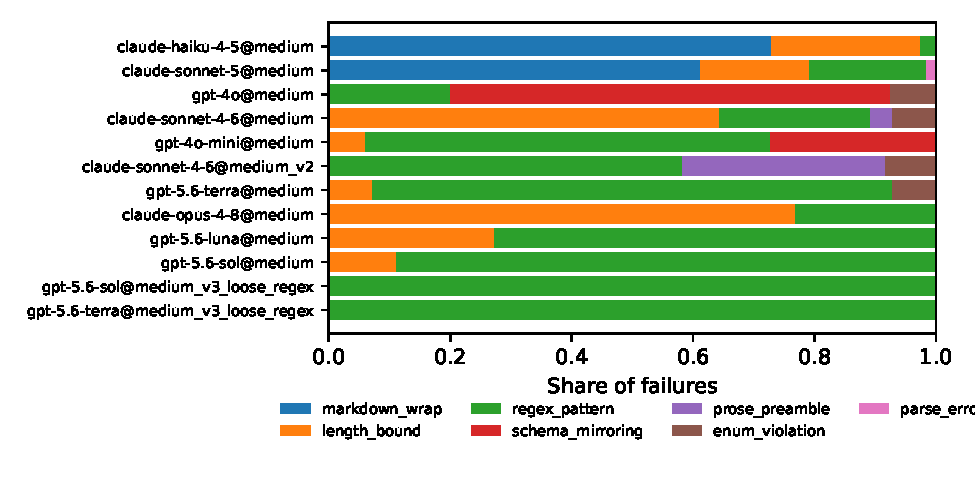
\includegraphics[width=0.92\linewidth]{generated/fig_profiles.pdf}
\caption{Composition of failures by model and schema tier, reporting
basis, ordered by failure rate.}
\label{fig:profiles}
\end{figure}

Grouping models by dominant category gives four observed profiles
(\cref{fig:profiles}): \cat{markdown\_wrap} for Haiku~4.5 and Sonnet~5;
\cat{regex\_pattern} for the three GPT-5.6 models and gpt-4o-mini;
\cat{length\_bound} for Opus~4.8 and Sonnet~4.6; and
\cat{schema\_mirroring} for gpt-4o. These are profiles read off the
dominant category, not clusters from any statistical procedure. They do
not follow vendor tier, since gpt-4o and gpt-4o-mini share a generation
but not a profile, and they do not follow rate: gpt-4o-mini, Sonnet~4.6
and gpt-4o fail at \pn{g.gpt-4o-mini@medium.rate},
\pn{g.claude-sonnet-4-6@medium.rate} and \pn{g.gpt-4o@medium.rate} with
three different dominant categories. Dominant shares for low-rate models
rest on few failures; Opus~4.8's \pn{g.claude-opus-4-8@medium.dominant_share}
share, for example, rests on \pn{g.claude-opus-4-8@medium.failures}
failures (Wilson \pn{g.claude-opus-4-8@medium.dominant_ci}).

Some categories are confined to particular models in our data.
\cat{schema\_mirroring} accounts for \pn{g.gpt-4o@medium.dominant_share}
of gpt-4o failures and was not observed in any GPT-5.6 configuration we
tested. \cat{markdown\_wrap} was not observed for Sonnet~4.6 across
\pn{m.claude-sonnet-4-6.attempts} attempts or Opus~4.8 across
\pn{m.claude-opus-4-8.attempts}, yet it accounts for
\pn{g.claude-sonnet-5@medium.dominant_share} of Sonnet~5 failures and
\pn{g.claude-haiku-4-5@medium.dominant_share} of Haiku~4.5 failures.
Haiku~4.5 and gpt-4o are each dominant in a category the other never
produces. Among the \pn{divergence.groups_qualifying} model--tier groups
with at least 20 failures, the largest difference between two groups in
the share of a single category is \pn{divergence.top.0.pp} percentage
points (\cref{app:divergence}).

\subsection{Profiles depend on the constraint surface}
\label{sec:results:surface}

\begin{table}[t]
\centering\small
\caption{Sonnet~4.6 at the medium and medium\_v2 tiers (HotpotQA). The
cells differ in size and are not paired by question.}
\label{tab:calibration}
\begin{tabular}{@{}lrrrr@{}}
\toprule
& \multicolumn{2}{c}{medium (178 att.)} & \multicolumn{2}{c}{medium\_v2 (324 att.)} \\
\cmidrule(lr){2-3}\cmidrule(lr){4-5}
Category & $n$ & rate & $n$ & rate \\
\midrule
\cat{length\_bound} & 18 & 10.1\% & 0 & 0.0\% \\
\cat{regex\_pattern} & 7 & 3.9\% & 14 & 4.3\% \\
\cat{prose\_preamble} & 1 & 0.6\% & 8 & 2.5\% \\
\cat{enum\_violation} & 2 & 1.1\% & 2 & 0.6\% \\
\midrule
All failures & 28 & 15.7\% & 24 & 7.4\% \\
\bottomrule
\end{tabular}

\end{table}

A profile is not a property of the model alone. Sonnet~4.6 is
\cat{length\_bound}-dominant at the medium tier
(\pn{calib.medium.length_bound} of \pn{calib.medium.failures} failures).
With the caps raised in medium\_v2, \cat{length\_bound} falls to
\pn{calib.medium_v2.length_bound}, \cat{regex\_pattern} becomes dominant
(\pn{calib.medium_v2.regex_pattern} of \pn{calib.medium_v2.failures}), and
the failure rate moves from \pn{calib.medium.rate} to
\pn{calib.medium_v2.rate} (\cref{tab:calibration}).

The error locations identify which caps were binding:
\pn{calib.field.coverage_notes.n} \code{coverage\_notes} values of
\pn{calib.field.coverage_notes.min}--\pn{calib.field.coverage_notes.max}
characters against the 250 cap (mean overrun
\pn{calib.field.coverage_notes.mean_overrun}, maximum
\pn{calib.field.coverage_notes.max_overrun}), \pn{calib.field.answer.n}
\code{answer} values of
\pn{calib.field.answer.min}--\pn{calib.field.answer.max} against 400 (mean
overrun \pn{calib.field.answer.mean_overrun}), and \pn{calib.field.fact.n} \code{fact} value of at most
\pn{calib.field.fact.max} characters against 400. These caps sat below the
lengths the model produced, not far below them. Because medium\_v2 is a
fresh generation, its result could in principle reflect changed output
rather than changed caps. Revalidating the \emph{stored} medium
completions against the medium\_v2 schema, \pn{calib.counterfactual_pass}
of \pn{calib.medium.length_bound} pass, so the elimination is mechanical.

Loosening the identifier character class is the contrasting case. On
HotpotQA, gpt-5.6-sol and gpt-5.6-terra produced
\pn{pert.medium.identifiers} violating identifiers under the baseline
pattern and \pn{pert.medium_v3_loose_regex.identifiers} under the
loosened pattern. Leading-digit violations such as the example in
\cref{sec:intro} went from \pn{pert.medium.leading_digit} to
\pn{pert.medium_v3_loose_regex.leading_digit}, as the loosened class
permits them. Length overflows against the retained 31-character ceiling
occurred under both patterns (\pn{pert.medium.length_overflow} and
\pn{pert.medium_v3_loose_regex.length_overflow}); with a handful of
failures per cell we do not interpret that change or the cell rates
(\cref{app:perturbation}). The relaxation removed the sub-cause it
addressed and did not address length overflow, which the
\cat{regex\_pattern} label conceals because the ceiling is written into
the pattern's quantifier.

\subsection{Formatting failures conceal content failures}
\label{sec:results:concealment}

\begin{table}[t]
\centering\small
\caption{Fence-strip revalidation of \cat{markdown\_wrap} failures,
reporting basis. \emph{Pure formatting} validates once the fence is
removed; \emph{compound} raises a further error.}
\label{tab:fence}
\begin{tabular}{@{}lrrr@{}}
\toprule
Model & Wrapped & Pure formatting & Compound \\
\midrule
\code{claude-haiku-4-5} & 640 & 290 (45.3\%) & 350 (54.7\%) \\
\code{claude-sonnet-5} & 41 & 37 (90.2\%) & 4 (9.8\%) \\
\midrule
All wrapped & 681 & 327 (48.0\%) & 354 (52.0\%) \\
\bottomrule
\end{tabular}

\end{table}

Because \cat{markdown\_wrap} takes precedence, it says nothing about what
lies inside the fence. We stripped the fence from every wrapped failure
and revalidated the payload (\cref{tab:fence}).
\pn{fence.reported.pure_share} validate; the rest raise a further error,
overwhelmingly on length: \pn{fence.reported.concealed.length_bound}
\cat{length\_bound}, \pn{fence.reported.concealed.regex_pattern}
\cat{regex\_pattern} and \pn{fence.reported.concealed.missing_field}
\cat{missing\_field}. The two wrapping models share a dominant category
but not what the wrapper hides: \pn{fence.claude-sonnet-5.compound} of
Sonnet~5's \pn{fence.claude-sonnet-5.n} wrapped failures are compound
(Wilson \pn{fence.claude-sonnet-5.compound_ci}), against
\pn{fence.claude-haiku-4-5.compound_share} of Haiku~4.5's
\pn{fence.claude-haiku-4-5.n}. Counting co-occurrence,
\cat{length\_bound} reaches \pn{reported.length_bound_incl_concealed}
instances against a primary count of \pn{reported.cat.length_bound}, so
primary counts are lower bounds on prevalence.

\begin{table}[t]
\centering\small
\caption{Prompt ablation on Haiku~4.5, HotpotQA, rates over attempts. The
last row counts length violations that are primary or concealed beneath a
fence.}
\label{tab:ablation}
\begin{tabular}{@{}lrrr@{}}
\toprule
& Baseline & Aggressive & Few-shot \\
\midrule
Attempts & 1{,}066 & 189 & 176 \\
\cat{markdown\_wrap} & 49.0\% & 33.9\% & 25.0\% \\
\cat{length\_bound} (primary) & 14.4\% & 16.4\% & 22.7\% \\
\cat{regex\_pattern} & 1.5\% & 2.1\% & 2.3\% \\
Failure rate & 64.9\% & 52.4\% & 50.0\% \\
\midrule
Length violations, primary + concealed & 37.8\% & 30.2\% & 36.9\% \\
\bottomrule
\end{tabular}

\end{table}

Concealment changes how a prompt ablation reads. We ran three
system-prompt variants on Haiku~4.5 on HotpotQA: the baseline, an
aggressive format instruction, and a few-shot prompt
(\cref{tab:ablation}). Wrapping falls from
\pn{ablation.baseline.markdown_wrap} of attempts to
\pn{ablation.few_shot.markdown_wrap}, a relative reduction of
\pn{ablation.delta.markdown_wrap_rel}, and the failure rate from
\pn{ablation.baseline.failure_rate} to \pn{ablation.few_shot.failure_rate}.
Primary \cat{length\_bound} rises from \pn{ablation.baseline.length_bound}
to \pn{ablation.few_shot.length_bound}, which read alone suggests
failures migrating from wrapping to length. But a suppressed fence can
expose a length violation that was already present. Counting primary and
concealed length violations together gives
\pn{ablation.baseline.length_bound_incl_concealed},
\pn{ablation.aggressive.length_bound_incl_concealed} and
\pn{ablation.few_shot.length_bound_incl_concealed}: the combined rate does
not rise as wrapping falls, so the rise in the primary share requires no
increase in over-long output. We do not interpret the differences among
the combined rates, including the lower aggressive figure; the variant
cells are much smaller than the baseline cell, were collected in separate
batches, and are not paired by question.

\section{Implications for Practice}
\label{sec:implications}
\label{sec:discussion} % kept so existing \cref{sec:discussion} still resolves

Three practices follow from the data, each at the scale of this corpus.

\paragraph{Strip fences, then revalidate and record what remains.}
Fence removal is a partial repair: it recovers the pure-formatting share
of wrapped failures, which ranged from most of Sonnet~5's to under half
of Haiku~4.5's (\cref{sec:results:concealment}). A pipeline that counts
fence removal as a fix would report the compound remainder as solved.
Because the parse error returned for a fenced output does not mention
the violation beneath it, the repair loop learns of that violation only
on a later attempt.

\paragraph{Represent identifier length separately when diagnosis matters.}
A \code{\{2,30\}} quantifier turns an over-long identifier into a pattern
violation, and the natural remedy for a pattern violation, loosening the
character class, leaves it untouched (\cref{sec:results:surface}). A
separate \code{max\_length} separates the causes at validation time.

\paragraph{Measure a field's observed length distribution before fixing its cap.}
Sonnet~4.6's dominant mode came from caps sitting modestly below its
output lengths, and Haiku~4.5's incomplete runs all ended on length. Such
a cap may still be a real downstream requirement; the measurement
identifies the mismatch the application must resolve, not that the cap
is wrong.

\paragraph{Will these modes persist?}
A reasonable objection is that providers are engineering these modes
away. Our cross-generation data are descriptive and do not isolate model
generation from other configuration differences, including collection
date, sampling parameters and endpoint. With that caveat, they point in
both directions: \cat{schema\_mirroring} dominates gpt-4o and was not
observed in the GPT-5.6 configurations we tested, while
\cat{markdown\_wrap} was not observed in Sonnet~4.6 and dominates
Sonnet~5 and Haiku~4.5. What differs across these models is which
category dominates. A vocabulary for the categories remains useful as the
distribution moves, which is a weaker claim than predicting that any
particular mode persists.

\section{Threats to Validity}
\label{sec:threats}

\paragraph{Construct validity.}
The taxonomy is an operational diagnostic for the prompt-and-validate
paradigm, not a complete account of structured-output failure. Primary
categories are single-valued, labels follow how a constraint is encoded
rather than what it intends (\cref{sec:setup:taxonomy}), and we quantify
co-occurrence only beneath fences. Classifier agreement is
development-set agreement from a single labeller who also wrote the
classifier. We evaluate conformance only, not whether extracted content
is correct. Among attempts whose model-level validators ran, no
cross-field violation occurred (\cref{app:crossfield}), but attempts
rejected earlier, including during JSON parsing, never reached those
checks, so the zero describes a filtered subset of the node-level
validators we implemented. Cross-node referential integrity, whether a
later node's identifiers appear in an earlier node's entities, is not
implemented in our schemas; it is expressible in Pydantic by passing the
earlier output as validation context
(\code{model\_validate\_json(data, context=\ldots)}) and is the natural
next measurement.

\paragraph{Internal validity.}
Repair attempts, which are conditioned on a prior failure, make up a
model-dependent share of each attempt rate; first-attempt rates and run
completion are reported separately for that reason
(\cref{app:breakdowns}). Every retry carries the validation error and no
condition retries without it, so the design does not separate the effect
of the feedback from that of a further attempt. Five models reject an
explicit temperature, and the Anthropic and OpenAI branches use
different token ceilings. Some questions were run more than once; keeping
only the earliest run per question changes any cell's failure rate by at
most \pn{robust.within_cell.max_abs_delta_pp} percentage points
(\cref{app:manifest}). The prompt-ablation variants were run after the
final baseline batch rather than interleaved with it and are not paired
by question.

\paragraph{External validity.}
The schemas are ours, and one ablation showed that a cap we set was
binding below the output lengths of one model; a different author would
produce a different distribution over categories, and the domain
comparison shows that a different task would too. We cover two vendors by
design, trading breadth for several generations and capability tiers per
vendor, which the within-family comparisons require; a third vendor or an
open-weights model may exhibit modes our taxonomy lacks. We do not
compare against constrained decoding or vendor structured-output modes
(\cref{sec:related}), so we make no claim about how often those
configurations would prevent the failures we report. Questions are fixed
dataset prefixes, the design is not fully crossed, and most failures in
this corpus come from a single model. Most endpoints returned an alias
rather than a pinned version, so later calls to the same identifier may
not reproduce these distributions.

\paragraph{Conclusion validity.}
Attempts are not independent, so all intervals are question-clustered
bootstrap intervals (\cref{sec:setup:basis}) that describe variability
over the observed question set, not over the benchmarks. No conclusion
depends on ordering models whose intervals overlap. We do not interpret
cells with a handful of failures, including the identifier-perturbation
cells and the combined length rates across prompt variants, and we treat
maximum-gap divergence statistics as secondary because they are selected
to be extreme (\cref{app:divergence}). The Haiku~4.5 FinanceBench cell
rests on \pn{c.claude-haiku-4-5@medium@financebench.questions} distinct
questions.

\section{Conclusion}
\label{sec:conclusion}

A validity rate for prompt-enforced structured output does not tell a
practitioner what failed or what a fix will change. Diagnosing a failure
requires keeping both the visible formatting failure and the schema
violation it may conceal; in this corpus, dropping either layer changes
the conclusion an engineer would draw about a repair, a schema change, or
a prompt change. Across
nine model configurations, those with similar rates fail
in different ways (RQ1); the dominant category moves when the binding constraints
change and differs between task domains for the same model (RQ2); and the
most common failure, markdown wrapping, conceals a length or pattern
violation often enough that reading primary labels alone misreads a
prompt ablation and misattributes what a repair loop leaves unrepaired
(RQ3). In both schema interventions we ran, whether a relaxation removed
a failure tracked the sub-cause beneath the label rather than the label
itself. Of the four practices we derive,
three are supported by these data; the fourth, building retry feedback
from the fence-stripped validation, follows from them but is untested. We release the classifier, raw
completions and annotation record so the corpus can be relabelled under
other definitions; the distribution over categories will move as models
change, and the vocabulary is meant to outlast it.


\ifanon\else
% Springer Nature requires a "Declarations" section before the references.
% Headings follow the sn-jnl template. VERIFY wording against EMSE's
% submission guidelines; edit anything that is not accurate.
\section*{Declarations}
\label{sec:declarations}

\bmhead{Funding} No funding was received for this work. API usage was
paid for by the author.

\bmhead{Competing interests}
% Keep the substance of your TMLR disclosure; edit as needed.
The author has no financial ties to OpenAI or Anthropic. The author works
as an on-site contractor at American Express through Data Systems
Integration Group; this work was carried out independently and is
unrelated to that role.

\bmhead{Ethics approval} Not applicable. The study involves no human
participants; the datasets used are public.

\bmhead{Data availability} The results database, raw completions,
annotations and question manifest are available at
\url{https://github.com/amitvermaknw/schema-enforcement}. FinanceBench
text is redistributed under CC~BY-NC~4.0 and HotpotQA questions under
CC~BY-SA~4.0 (see \code{DATA\_LICENSES.md}).

\bmhead{Code availability} The harness, classifier and analysis scripts
are available in the same repository.

\bmhead{Use of AI tools}
% Springer Nature policy: LLMs cannot be authors; document their use.
The author used large language model assistants (Claude) for writing,
editing and coding assistance. All experiments were designed, run and
verified by the author; every number reported is generated by scripts
from the released results database.

\bmhead{Author contributions} Sole author: conceptualisation,
methodology, software, analysis and writing.

\fi

\begin{appendices}
\section{Cell Manifest, Versions and Sampling}
\label{app:manifest}

\begin{table}[h]
\centering\scriptsize
\caption{All cells, baseline prompt. Pilot cells (fewer than 30 runs) are
excluded from the reporting basis.}
\begin{tabular}{@{}lllrrrl@{}}
\toprule
Model & Tier & Domain & Runs & Att. & Fail & Status \\
\midrule
\code{claude-haiku-4-5} & medium & financebench & 32 & 263 & 186 &  \\
\code{claude-haiku-4-5} & medium & hotpotqa & 194 & 1{,}066 & 692 &  \\
\code{claude-opus-4-8} & medium & financebench & 30 & 101 & 11 &  \\
\code{claude-opus-4-8} & medium & hotpotqa & 54 & 164 & 2 &  \\
\code{claude-sonnet-4-6} & medium & hotpotqa & 50 & 178 & 28 &  \\
\code{claude-sonnet-5} & medium & financebench & 30 & 114 & 24 &  \\
\code{claude-sonnet-5} & medium & hotpotqa & 52 & 199 & 43 &  \\
\code{gpt-4o} & medium & hotpotqa & 70 & 250 & 40 &  \\
\code{gpt-4o-mini} & medium & financebench & 5 & 28 & 13 & pilot (excluded) \\
\code{gpt-4o-mini} & medium & hotpotqa & 70 & 242 & 33 &  \\
\code{gpt-5.6-luna} & medium & financebench & 30 & 97 & 7 &  \\
\code{gpt-5.6-luna} & medium & hotpotqa & 55 & 169 & 4 &  \\
\code{gpt-5.6-sol} & medium & financebench & 30 & 96 & 6 &  \\
\code{gpt-5.6-sol} & medium & hotpotqa & 52 & 159 & 3 &  \\
\code{gpt-5.6-terra} & medium & financebench & 30 & 98 & 8 &  \\
\code{gpt-5.6-terra} & medium & hotpotqa & 54 & 168 & 6 &  \\
\code{claude-sonnet-4-6} & medium\_v2 & hotpotqa & 100 & 324 & 24 &  \\
\code{gpt-5.6-luna} & medium\_v3\_loose\_regex & hotpotqa & 2 & 6 & 0 & pilot (excluded) \\
\code{gpt-5.6-sol} & medium\_v3\_loose\_regex & hotpotqa & 50 & 155 & 5 &  \\
\code{gpt-5.6-terra} & medium\_v3\_loose\_regex & hotpotqa & 50 & 154 & 4 &  \\
\bottomrule
\end{tabular}

\end{table}

\paragraph{Sampling.}
HotpotQA questions are the first records of the validation split in the
distractor configuration, in dataset order; FinanceBench questions are the
first records of the train split, with evidence truncated to 2{,}000
characters and a truncation marker inserted. There is no shuffle and no
seed.

\paragraph{Resolved versions.}
Anthropic models and the GPT-5.6 family return the requested alias
unchanged. \code{gpt-4o} resolves to \code{gpt-4o-2024-08-06} and
\code{gpt-4o-mini} to \code{gpt-4o-mini-2024-07-18}. Version capture was
added after the first sweeps: \pn{versions.gpt-4o.precapture} of
\pn{versions.gpt-4o.attempts} \code{gpt-4o} attempts and
\pn{versions.gpt-4o-mini.precapture} of \pn{versions.gpt-4o-mini.attempts}
\code{gpt-4o-mini} attempts on the reporting basis predate it.

\paragraph{Repeated questions.}
The Haiku~4.5 HotpotQA baseline cell contains \pn{robust.cell.runs} runs
over \pn{robust.cell.questions} distinct questions. Restricting it to the
earliest run of each question gives a failure rate of
\pn{robust.one_run.rate} (\pn{robust.one_run.failures} of
\pn{robust.one_run.attempts}) against \pn{robust.cell.rate}
(\pn{robust.cell.failures} of \pn{robust.cell.attempts}) for the full cell.

\paragraph{Zero-length completion.}
One attempt (\pn{zero_length.model}, \pn{zero_length.node} node) returned
an empty completion with \pn{zero_length.output_tokens} output tokens,
equal to the configured ceiling. It is classified \cat{parse\_error}. The
stop reason was not logged; the record is consistent with the output
budget being exhausted before any text block was emitted.

\section{Schemas and Prompts}
\label{app:schemas}

The three schema tiers and three prompt variants are reproduced from the
released code.

\IfFileExists{code/medium.py}{\lstinputlisting[language=Python,caption={Medium tier schema}]{code/medium.py}}{\emph{[Copy src/schemaeval/schemas/medium.py to paper/code/medium.py.]}}

\IfFileExists{code/prompts.py}{\lstinputlisting[language=Python,caption={Prompt variants}]{code/prompts.py}}{\emph{[Copy src/schemaeval/prompts.py to paper/code/prompts.py.]}}

The medium\_v2 tier differs only in the three character caps and the
medium\_v3\_loose\_regex tier only in \code{CANONICAL\_ID\_PATTERN}.

\section{Classifier Validation}
\label{app:classifier}

\paragraph{Provenance.}
Hand labelling was performed against an earlier classifier in which
Pydantic error-type mapping preceded the behavioural predicates.
Schema-mirrored outputs were consequently labelled \cat{missing\_field}
and prose-preamble outputs \cat{parse\_error}. We corrected the order and
reclassified the full corpus from stored completions and error details;
the released \code{errors.py} and \code{reclassify\_all.py} reproduce
every label.

\paragraph{Agreement.}
The sample was drawn from all \pn{full.failures} failures in the corpus,
including pilot cells and prompt variants. \Cref{tab:validation} reports
precision and recall of the corrected classifier against the \emph{blind}
human labels. The four disagreements were adjudicated as labelling
errors: three outputs labelled \cat{enum\_violation} carried a
\code{string\_pattern\_mismatch} on an identifier, and one labelled
\cat{markdown\_wrap} contained no fence. We headline blind agreement
because adjudication uses evidence the labeller did not consult.

\begin{table}[h]
\centering\small
\caption{Corrected classifier against blind human labels
($n=\pn{validation.n}$), full corpus frame.}
\label{tab:validation}
\begin{tabular}{@{}lrll@{}}
\toprule
Category & Predicted & Precision & Recall \\
\midrule
\cat{markdown\_wrap} & 25 & 25/25 & 25/26 \\
\cat{length\_bound} & 30 & 30/30 & 30/30 \\
\cat{regex\_pattern} & 30 & 27/30 & 27/27 \\
\cat{schema\_mirroring} & 42 & 42/42 & 42/42 \\
\cat{prose\_preamble} & 9 & 8/9 & 8/8 \\
\cat{enum\_violation} & 8 & 8/8 & 8/11 \\
\bottomrule
\end{tabular}

\end{table}

\paragraph{Corpus screens.}
Because the sample is stratified by predicted label, it cannot establish
corpus recall. For the Stage-1 categories we screened every failure in
the full corpus with predicates broader than the detectors. A fence at
any position matches \pn{screen.fence_any.matches} failures, of which
\pn{screen.fence_any.markdown_wrap} are classified \cat{markdown\_wrap}
and \pn{screen.fence_any.prose_preamble} \cat{prose\_preamble} (prose
before a later fence). A \code{"properties"} key matches
\pn{screen.properties.matches} failures, of which
\pn{screen.properties.schema_mirroring} are classified
\cat{schema\_mirroring}; this screen tests one meta-keyword where the
detector requires two, so it bounds recall only among failures containing
that key. An opening character other than a brace, bracket or fence
matches \pn{screen.nonjson_opener.matches} non-empty failures, of which
\pn{screen.nonjson_opener.prose_preamble} are \cat{prose\_preamble}.

\section{Identifier Perturbation}
\label{app:perturbation}

\begin{table}[h]
\centering\small
\caption{Sub-causes of violating identifiers in \cat{regex\_pattern}
failures, gpt-5.6-sol and gpt-5.6-terra, HotpotQA. Counts are
identifiers, not attempts.}
\label{tab:perturbation}
\begin{tabular}{@{}lrr@{}}
\toprule
Sub-cause & Baseline pattern & Loosened pattern \\
\midrule
Leading digit & 4 & 0 \\
Length overflow & 4 & 10 \\
Unicode contamination & 0 & 1 \\
Other character & 0 & 0 \\
\midrule
Violating identifiers & 8 & 11 \\
\bottomrule
\end{tabular}

\end{table}

The baseline tier uses \idpattern{} and the perturbed tier \idpatternloose{};
both retain the 31-character ceiling, and the loosened pattern also
governs the supporting-identifier check inside the answer validator.
Sub-causes are assigned mechanically per identifier: non-ASCII characters,
a leading digit not admitted by the first-character class, other
characters outside the class, and length outside 3--31. The cells hold
\pn{pert.medium.gpt-5.6-sol.failures} and
\pn{pert.medium.gpt-5.6-terra.failures} failures under the baseline
pattern and \pn{pert.medium_v3_loose_regex.gpt-5.6-sol.failures} and
\pn{pert.medium_v3_loose_regex.gpt-5.6-terra.failures} under the loosened
pattern, too few to support rates or shares. The single Unicode case
under the loosened pattern is an otherwise lowercase band name with a
non-Latin combining mark inserted.

\section{Per-Domain and First-Attempt Breakdowns}
\label{app:breakdowns}

\begin{table}[h]
\centering\scriptsize
\caption{Per-cell results, reporting basis.}
\begin{tabular}{@{}lllrrrl@{}}
\toprule
Model & Tier & Domain & Att. & Rate & Att./run & Dominant \\
\midrule
\code{claude-haiku-4-5} & medium & financebench & 263 & 70.7\% & 8.22 & \cat{markdown\_wrap} \\
\code{claude-haiku-4-5} & medium & hotpotqa & 1{,}066 & 64.9\% & 7.96 & \cat{markdown\_wrap} \\
\code{claude-opus-4-8} & medium & financebench & 101 & 10.9\% & 3.37 & \cat{length\_bound} \\
\code{claude-opus-4-8} & medium & hotpotqa & 164 & 1.2\% & 3.04 & \cat{regex\_pattern} \\
\code{claude-sonnet-4-6} & medium & hotpotqa & 178 & 15.7\% & 3.56 & \cat{length\_bound} \\
\code{claude-sonnet-4-6} & medium\_v2 & hotpotqa & 324 & 7.4\% & 3.24 & \cat{regex\_pattern} \\
\code{claude-sonnet-5} & medium & financebench & 114 & 21.1\% & 3.80 & \cat{length\_bound} \\
\code{claude-sonnet-5} & medium & hotpotqa & 199 & 21.6\% & 3.83 & \cat{markdown\_wrap} \\
\code{gpt-4o} & medium & hotpotqa & 250 & 16.0\% & 3.57 & \cat{schema\_mirroring} \\
\code{gpt-4o-mini} & medium & hotpotqa & 242 & 13.6\% & 3.46 & \cat{regex\_pattern} \\
\code{gpt-5.6-luna} & medium & financebench & 97 & 7.2\% & 3.23 & \cat{regex\_pattern} \\
\code{gpt-5.6-luna} & medium & hotpotqa & 169 & 2.4\% & 3.07 & \cat{regex\_pattern} \\
\code{gpt-5.6-sol} & medium & financebench & 96 & 6.2\% & 3.20 & \cat{regex\_pattern} \\
\code{gpt-5.6-sol} & medium & hotpotqa & 159 & 1.9\% & 3.06 & \cat{regex\_pattern} \\
\code{gpt-5.6-sol} & medium\_v3\_loose\_regex & hotpotqa & 155 & 3.2\% & 3.10 & \cat{regex\_pattern} \\
\code{gpt-5.6-terra} & medium & financebench & 98 & 8.2\% & 3.27 & \cat{regex\_pattern} \\
\code{gpt-5.6-terra} & medium & hotpotqa & 168 & 3.6\% & 3.11 & \cat{regex\_pattern} \\
\code{gpt-5.6-terra} & medium\_v3\_loose\_regex & hotpotqa & 154 & 2.6\% & 3.08 & \cat{regex\_pattern} \\
\bottomrule
\end{tabular}

\end{table}

\begin{table}[h]
\centering\scriptsize
\caption{First-attempt validity by node. The denominator is the number of
runs that reached the node, which depends on upstream success; the
identify node is the only unconditioned comparison.}
\begin{tabular}{@{}lllrr@{}}
\toprule
Model & Tier & Node & Reached & First-attempt valid \\
\midrule
\code{claude-haiku-4-5} & medium & answer & 143 & 0.0\% \\
\code{claude-haiku-4-5} & medium & gather & 166 & 0.0\% \\
\code{claude-haiku-4-5} & medium & identify & 166 & 0.0\% \\
\code{claude-opus-4-8} & medium & answer & 84 & 89.3\% \\
\code{claude-opus-4-8} & medium & gather & 84 & 100.0\% \\
\code{claude-opus-4-8} & medium & identify & 84 & 96.4\% \\
\code{claude-sonnet-4-6} & medium & answer & 50 & 84.0\% \\
\code{claude-sonnet-4-6} & medium & gather & 50 & 82.0\% \\
\code{claude-sonnet-4-6} & medium & identify & 50 & 82.0\% \\
\code{claude-sonnet-4-6} & medium\_v2 & answer & 100 & 96.0\% \\
\code{claude-sonnet-4-6} & medium\_v2 & gather & 100 & 96.0\% \\
\code{claude-sonnet-4-6} & medium\_v2 & identify & 100 & 84.0\% \\
\code{claude-sonnet-5} & medium & answer & 82 & 86.6\% \\
\code{claude-sonnet-5} & medium & gather & 82 & 76.8\% \\
\code{claude-sonnet-5} & medium & identify & 82 & 64.6\% \\
\code{gpt-4o} & medium & answer & 70 & 58.6\% \\
\code{gpt-4o} & medium & gather & 70 & 100.0\% \\
\code{gpt-4o} & medium & identify & 70 & 84.3\% \\
\code{gpt-4o-mini} & medium & answer & 70 & 85.7\% \\
\code{gpt-4o-mini} & medium & gather & 70 & 100.0\% \\
\code{gpt-4o-mini} & medium & identify & 70 & 78.6\% \\
\code{gpt-5.6-luna} & medium & answer & 85 & 96.5\% \\
\code{gpt-5.6-luna} & medium & gather & 85 & 100.0\% \\
\code{gpt-5.6-luna} & medium & identify & 85 & 90.6\% \\
\code{gpt-5.6-sol} & medium & answer & 82 & 98.8\% \\
\code{gpt-5.6-sol} & medium & gather & 82 & 100.0\% \\
\code{gpt-5.6-sol} & medium & identify & 82 & 90.2\% \\
\code{gpt-5.6-sol} & medium\_v3\_loose\_regex & answer & 50 & 98.0\% \\
\code{gpt-5.6-sol} & medium\_v3\_loose\_regex & gather & 50 & 100.0\% \\
\code{gpt-5.6-sol} & medium\_v3\_loose\_regex & identify & 50 & 92.0\% \\
\code{gpt-5.6-terra} & medium & answer & 84 & 98.8\% \\
\code{gpt-5.6-terra} & medium & gather & 84 & 100.0\% \\
\code{gpt-5.6-terra} & medium & identify & 84 & 84.5\% \\
\code{gpt-5.6-terra} & medium\_v3\_loose\_regex & answer & 50 & 100.0\% \\
\code{gpt-5.6-terra} & medium\_v3\_loose\_regex & gather & 50 & 100.0\% \\
\code{gpt-5.6-terra} & medium\_v3\_loose\_regex & identify & 50 & 92.0\% \\
\bottomrule
\end{tabular}

\end{table}

\section{Model-Level Constraints}
\label{app:crossfield}

Model validators run only after every field-level constraint passes.
On the reporting basis, \pn{crossfield.reached} attempts reached them:
\pn{crossfield.validated} that validated and \pn{modellevel.violations}
that passed field validation and failed the per-item
supporting-identifier check in the answer validator. That check follows
the confidence-bucket check in the same method, so those attempts also
passed it. No attempt matched any of the four cross-field messages
(\pn{crossfield.violations} violations). The remaining
\pn{crossfield.not_reached} failures did not reach the validators; many
failed during JSON parsing. Each node tests only its own checks: two
cross-field checks in identify, one in gather, and one cross-field plus
one per-item pattern check in answer.

\section{Divergence Metric}
\label{app:divergence}

For each pair of model--tier groups and each category we take the
absolute difference in the share of the group's failures held by that
category. Groups pool task domains and use the reporting basis; of
\pn{divergence.groups_total} groups with any failure,
\pn{divergence.groups_qualifying} have at least 20 failures, giving
\pn{divergence.pairs} pairs. The two largest values arise on different
categories from opposite vendors, \pn{divergence.top.0.pp} and
\pn{divergence.runner_up_category_pp} points, and differ by
\pn{divergence.gap_pp} points, so we attach no significance to their order. Without the threshold the maximum
is \pn{divergence.unrestricted.top.0.pp} points, but it involves a group
with very few failures.

\begin{table}[h]
\centering\small
\caption{Largest category-share differences among qualifying groups.}
\begin{tabular}{@{}lllr@{}}
\toprule
Category & Group A & Group B & pp \\
\midrule
markdown\_wrap & \code{claude-haiku-4-5@medium} & \code{claude-sonnet-4-6@medium} & 72.9 \\
markdown\_wrap & \code{claude-haiku-4-5@medium} & \code{claude-sonnet-4-6@medium\_v2} & 72.9 \\
markdown\_wrap & \code{claude-haiku-4-5@medium} & \code{gpt-4o@medium} & 72.9 \\
markdown\_wrap & \code{claude-haiku-4-5@medium} & \code{gpt-4o-mini@medium} & 72.9 \\
schema\_mirroring & \code{claude-haiku-4-5@medium} & \code{gpt-4o@medium} & 72.5 \\
schema\_mirroring & \code{claude-sonnet-4-6@medium} & \code{gpt-4o@medium} & 72.5 \\
schema\_mirroring & \code{claude-sonnet-4-6@medium\_v2} & \code{gpt-4o@medium} & 72.5 \\
schema\_mirroring & \code{claude-sonnet-5@medium} & \code{gpt-4o@medium} & 72.5 \\
\bottomrule
\end{tabular}

\end{table}

\end{appendices}

\bibliography{references}

\end{document}